 \documentclass[letterpaper,12pt,titlepage]{article}

\usepackage[letterpaper, margin=1in]{geometry}
\usepackage{authblk}
\usepackage{amsmath}
\usepackage{amsfonts}
\usepackage{listings}
\usepackage{graphicx}
\usepackage{braket}
\usepackage{appendix}
\usepackage[justification=justified]{subcaption}
\usepackage{cite}
\usepackage{titlepic}
\usepackage{comment}
\usepackage{multicol}
\usepackage{multienum}
\usepackage{color}
\usepackage[normalem]{ulem}
\usepackage[hidelinks]{hyperref}

\graphicspath{{figures/}}
\newcommand{\yz}[1]{\textcolor{blue}{YZ: #1}}

\lstset{
  columns=flexible,
  basicstyle=\small\ttfamily,
  mathescape=true,
  escapeinside=||
}
\providecommand{\versionnumber}{2.0.2}
\newenvironment{multiitem}{%
  \multienumerate\renewcommand{\labelname}{\textbullet}%
}{%
  \endmultienumerate%
}

\title{Non-adiabatic EXcited-state Molecular Dynamics (NEXMD) Reference Manual\\ Version \versionnumber}
\titlepic{
\includegraphics[width=\textwidth]{NEXMD.pdf}}
\date{}

\begin{document}
\maketitle
\tableofcontents

\newpage
\section{Introduction}

NEXMD, from Non-adiabatic EXcited state Molecular Dynamics\cite{malone2020nexmd,nelson2020non}, is a software package designed for simulating the non-radiative electronic relaxation taking place in a molecular system after a photo-excitation. The intricate mechanisms taking place between the excited states manifold underpins processes in nature such as vision\cite{polli2010conical} or photosynthesis\cite{scholes2017using}. A detailed understanding of these mechanisms have also allowed a wide range of applications including but not limited to organic light emitting diodes\cite{salehi2019recent}, photovoltaics\cite{wang2014photodegradation,wolfer2014solution,zhugayevych2015theoretical}, field-effect transistors\cite{sirringhaus2000high,lee2016highly}, sensors\cite{satishkumar2007reversible,maksimov2019genetically,li2019perylene,wilson2008photoactive,singer2022unravelling}, photocatalysts\cite{romero2016organic} and solar cells\cite{bredas2009molecular,schmidt2011moving}. The complex excited state electronic structure arising from strong electronic correlations and low dimensionality\cite{tretiak2002conformational}, combined with delocalized and polarizable $\pi$-electrons are key for the generation of mobile charge carriers\cite{cao1999improved}. Such systems typically undergo an efficient non-radiative relaxation\cite{kasha1950characterization} that can take place through several nonadiabatic pathways leading to overall dissipation of an excess of electronic energy into heat. In this context, many physical processes such as internal conversion\cite{robb2000computational}, energy transfer\cite{jiang2017light}, charge separation\cite{huix2015concurrent,bredas2004charge}, exciton self-trapping\cite{adamska2014self} or vibronic coherences\cite{freixas2020vibronic,keefer2021monitoring,freixas2022ultrafast} can be of relevance.

NEXMD is able to simulate these processes from a full-atom perspective treating molecules that have a few hundreds of atoms, including a few dozens of excited states and for a few picoseconds. The electronic structure is based in the Colective Electronic Oscillator (CEO) method\cite{tretiak2002density}, considering Configuration Interaction Singles\cite{thouless2014quantum} or the Time-Dependent Hartree-Fock (TDHF)\cite{jorgensen1975molecular,mclachlan1964time} combined with semiempirical Hamiltonians models. The initial implementation (NEXMD Version 1.0), included the Trajectory Surface Hopping approach\cite{tully1990molecular}. Recent implementations have added Ehrenfest dynamics\cite{fernandez2016non} and the Ab-Inition Multiple Cloning sampling for Multiconfigurational Ehrenfest\cite{freixas2018ab}. These methods in combination with other features present in NEXMD allow a comprehensive investigation of a wide range of processes and systems, including but not limited to polymers\cite{clark2012femtosecond,oldani2014modeling,ondarse2014computational,alfonso2016interference,sifain2018photoexcited,ondarse2018let,mukazhanova2023impact}, dendrimers\cite{freixas2022ultrafast,ondarse2016ultrafast,galindo2015dynamics,fernandez2012shishiodoshi,soler2012analysis,ondarse2018energy,freixas2019photoinduced,bonilla2023impact}, nanorings and nanobelts\cite{franklin2017phonon,oldani2017photoinduced,rodriguez2018modification,franklin2016carbon,freixas2022infinitene,negrin2023photoexcited}, light harvesting complexes\cite{bricker2015non,shenai2015internal,zheng2017photoinduced} and energetic materials\cite{greenfield2015photoactive,nelson2016ultrafast,lystrom2018site}.

This document is a user manual covering technical details required for using NEXMD, such as available features, compilation and execution, input file extensive description and output files formatting. It also contains a section with input files examples intended to be used as templates for the specific features available within NEXMD. This manual is not intended to cover the theoretical background supporting the features of NEXMD. The interested reader can use instead a recent extensive review on NEXMD\cite{nelson2020non} or specialized papers on the development of a given feature or application. While this manual is a useful guide for the new user, more guided tutorials (specific to particular use cases) are available elsewhere.

\newpage
\section{NEXMD Main Features}

NEXMD/NEXMD v2 have been principally developed to perform on-the-fly non-adiabatic excited state molecular dynamics simulations at TDHF or CIS level of electronic structure using semiempirical Hamiltonians. It also comprises several features that are useful when analyzing the photophysics of a molecular system. In this section we enumerate some of NEXMD features and corresponding input keywords, while the full list and the details for configuring the corresponding input parameters can be found in the Section \ref{Input_file}.

\begin{itemize}
\item Electronic structure single point is done when both the classical steps \verb+n_class_steps+ and the optimization cycles \verb+maxcyc+ are set to zero. In the standard output (usually denoted as \verb+md.out+), NEXMD will write the ground state and excited state energies along with the corresponding electric transition dipole moments and oscillator strengths. Furthermore the following options are available:
    \begin{itemize}
        \item Mulliken charges: Can be set with \verb+printcharges+.
        \item Transition dipole moments between excited states: Can be set with \verb+calcxdens+.
        \item Transition density plots: Can be set with \verb+out_data_cube+. This option will generate a set of \verb+.DATA+ files that can be converted to \verb+.cube+ files and plotted with any standard chemical software. 
    \end{itemize}

\item Optimization can be done for the ground state or any excited state by setting the variable \verb+maxcyc+ to any value greater than zero. The number of classical steps has to be reduced to zero otherwise an error will show up in the standard output. 

\item Hessian and normal mode calculations can be set with \verb+do_nm+. Both the number of classical steps \verb+n_class_steps+ and the optimization cycles \verb+maxcyc+ have to be set to zero.

\item Molecular dynamics can be set when the number of classical steps \verb+n_class_steps+ is set to a value greater than zero. NEXMD includes the following types of molecular dynamics:
    \begin{itemize}
        \item Ground state molecular dynamics is performed when the initial excited state \verb+exc_state_init+ is set to zero. If the number of excited states to calculate \verb+\n_exc_states_propagate+ is set to number greater than zero, the energies and transition dipole moments of the corresponding states will be calculated along the ground state dynamics.
        \item Adiabatic excited state dynamics can be activated by setting the initial excited state \verb+exc_state_init+ to a value greater than zero and the Born-Oppenheimer flag \verb+bo_dynamics_flag+ to one. The number of excited states to propagate in the input variable \verb+n_exc_states_propagate+ has to be greater than \verb+exc_state_init+.
        \item Non-adiabatic excited state dynamics can be activated setting the initial excited state \verb+exc_state_init+ to a value greater than zero and the Born-Oppenheimer flag \verb+bo_dynamics_flag+ to zero. By default the non-adiabatic dynamic method is the trajectory surface hopping. The type of non-adiabatic molecular dynamics can also be set to perform Ehrenfest or Ab-initio Multiple Cloning dynamics by means of the variable \verb+NAMD_type+.
    \end{itemize}

\item Langevin thermostat can be activated setting \verb+therm_type+ to one for any of the types of molecular dynamics, although it is advised to only use it for ground state dynamics. 

\item Implicit solvation schemes are available by setting the input variable \verb+solvent_model+. Vertical excitation and state specific methods are not advised for non-adiabatic dynamics since instantaneous quantum transitions instantaneously change the charge density, which in turn instantly changes polarized solvent field leading to an unphysical sudden change of the excited state solutions.

\item Constraints can be activated between atom distances or for generalized directions, e.g. normal modes. Only one type of constraint is advised to be used in a calculation.
    \begin{itemize}
        \item Constraints for atom distances can be activated with the input variable \verb+npc+.
        \item Constraints for generalized directions can be activated with the input variable \verb+nmc+.
    \end{itemize}

\end{itemize}

\newpage
\section{Compiling NEXMD}

Expanding upon the readme, the \verb+Makefile+ for \verb+NEXMD+ is handwritten for both \verb+GNU+ and \verb+Intel+ Fortran compilers and libraries with their default names and locations. 
By default a serial binary is compiled and libraries are statically linked.
The \verb+Makefile+
should work for most standard systems (sometimes only after loading
the relevant compiler and library module) 
%please contact !email! if that is not the case.

Calling the \verb+make+ command in the NEXMD directory will call the default \verb+Intel+ Fortran compiler with \verb+Intel+ MKL libraries, equivalent to calling 
\verb+make all+ and \verb+make ic_mkl+

The other tested option is \verb+make gnu+ which will call the default \verb+GNU+ Fortran compiler with BLAS and LAPack libraries in their default
location.

There are commented out options, as examples for tinkering with
the Makefile for advanced users. 

\subsection{Stack size}

Similar to most programs, if \verb+nexmd.exe+ has insufficient space on the
stack it will crash with no useful error messages.

Before running calculations, it is useful to ensure there is sufficient
stack size, for \verb+BASH+:
\begin{lstlisting}[mathescape=false,escapeinside={(*@}{@*)}]
ulimit -s unlimited
\end{lstlisting}
or
\begin{lstlisting}[mathescape=false,escapeinside={(*@}{@*)}]
ulimit -s hard
\end{lstlisting}

This may require super-user permissions.

\subsection{Avoiding edits to the Makefile}
For \verb+BASH+,
the default \verb+Makefile+ can be used with non-default compiler locations by adding these locations to the path:
\begin{lstlisting}[mathescape=false,escapeinside={(*@}{@*)}]
export PATH = <NEXMD directory>:$PATH
\end{lstlisting}

For \verb+BASH+,
it may be possible that custom libraries can be softlinked to the main repository.
\begin{lstlisting}[mathescape=false,escapeinside={(*@}{@*)}]
ln -s <custom library file> <NEXMD directory>/<special_lib>
\end{lstlisting}

\subsection{Advance configuration}

Advanced users on custom systems may find that they need NEXMD compiled with custom compilers and libraries outside the default location. 
The \verb+Makefile+ contains empty variables under the flag \verb+custom+
for such custom compilers and libraries; for complete flexibility.
%Please contact !email! for assistance.

\subsection{Tests after compiling}
\verb+<NEXMD directory>/tests+ contains template input and bash scripts for NEXMD2 calculations on benzene;
\verb+<NEXMD directory>/tests/reference+ contains reference output of the tests.

\newpage
\section{Running NEXMD}

NEXMD is a command-line program which always uses a main input file named \verb+input.ceon+, and rarely requires additional input files. The typical workflow is constructing the input in a fresh directory and calling the program as:

\vspace{0.5cm}
\verb+/path_to_nexmd_bin/nexmd.exe > md.out &+
\vspace{0.5cm}

and it is possible to use a main input file with a non-standard name with

\vspace{0.5cm}
\verb+/path_to_nexmd_bin/nexmd.exe < custom_input.ceon > md.out &+
\vspace{0.5cm}
.

Several output files (in addition to the standard output which above is written to \verb+md.out+) will be generated depending on the input parameters. More details about the output files content and format can be found in section 6 of this manual.

Example NEXMD \verb+input.ceon+ files with the expected output are present in the test directory found at
\verb+<NEXMD directory>/tests+. These examples cover most of the features present in NEXMD. It is advised to use these examples to test the NEXMD immediately after compilation. Furthermore, when building a new \verb+input.ceon+ file, it is also advised to use as template one of the \verb+input.ceon+ in the \verb+tests+ directory or in this manual, and modify only the necessary parameters for activating the desired features. This minimal changes are intended to avoid combinations of input keywords that are not benchmarked, not physically justified, or are partially ignored by the sequential reading of keywords as a safeguard to reduce wasting computational resources.

It is also important to notice that there are three mutually-exclusive calculations that NEXMD can perform, enforced by the sequential reading of the main input file. These are optimization, normal modes calculation and molecular dynamics propagation. A main input file suggesting to perform more than one of these calculations will result in an error written to standard output.

Among NEXMD output files, there is one named \verb+restart.out+ written for all the molecular dynamics flavors, which is an input file for restarting the dynamics. If such file is present, NEXMD will restart the simulation from the last molecular dynamics step. The program can be called in a similar way:

\vspace{0.5cm}
\verb+/path_to_nexmd_bin/nexmd.exe < input.ceon >> md.out &+
\vspace{0.5cm}

or

\vspace{0.5cm}
\verb+/path_to_nexmd_bin/nexmd.exe < restart.out >> md.out &+
\vspace{0.5cm}

Note the \verb+>>+ before \verb+md.out+ to append instead of overwriting the standard output file. More details about restarting can be found in section 7 of this manual.

The usual NEXMD workflow when doing research can be followed in Figure \ref{general_flow}. Each of these steps is either an individual run, a set of individual runs, or the analysis of a set of output files.

\begin{figure}[ht]
	\centering
	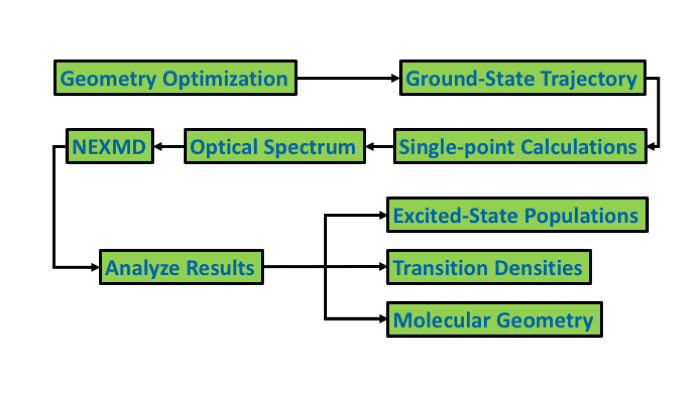
\includegraphics[scale=.6]{general_procedure.png}
	\caption{\small A schematic of the general procedure for simulating non-adiabatic dynamics.}\label{general_flow}
\label{genproc}
\end{figure}

\newpage
\section{The input file}\label{Input_file}

The contents of the input file for \verb+NEXMD+ can be categorized into blocks: 
\verb+&qmmm+ for geometry optimization, ground-state parameters, excited-state parameters, and solvent models; \verb+&moldyn+ for molecular dynamics, thermostats, and constraints; \verb+&pairs+ and \verb+&modes+ for specifying constraints; \verb+&coord+ for initial geometries; \verb+&veloc+ for initial velocity and \verb+&coeff+ for excited-state coefficients.  All input parameters are overviewed here, the numerical values in square brackets are default parameters.
\vspace{0.5cm}

\begin{lstlisting}[mathescape=false,escapeinside={(*@}{@*)}]
&qmmm
   !***** Geometry Optimization
\end{lstlisting}
The following section contains input parameters pertaining to geometry optimization.
\begin{lstlisting}[mathescape=false,escapeinside={(*@}{@*)}]
   maxcyc=0, ! Number of cycles for geometry optimization [0]
   ntpr=1, ! Print results every ntpr cycles [1]
   grms_tol=1.0d-2, ! Tolerance in eV/A (derivatives) [1.0d-2]
\end{lstlisting}
\begin{itemize}
\item \verb+maxcyc+ sets the maximum number of cycles for geometry optimization.  If the number of cycles reaches \verb+maxcyc+, an error message reads: \verb+Maximum+ \verb+number+ \verb+of+ \verb+iterations+ \verb+reached+ \verb+without+ \verb+convergence+.  Therefore,  to optimize geometry, \verb+maxcyc+ must be set to a sufficiently large number greater than zero.  If the geometry reaches the maximum number of cycles, you must review the situation carefully to determine if the input geometry was appropriate or if \verb+grms_tol+ (shown below) was set too low.  A negative \verb+maxcyc+ is treated as \verb+0+. All files written according to the corresponding verbosity will be written for the optimized geometry.
\item \verb+ntpr+ sets how often results for geometry optimization are printed to the standard output file.  The output of the iteration is written as \verb+iter+, \verb+energy+ in eV, and \verb+rms+ \verb+gradient+ in eV per \AA.  The latter quantity is explained in \verb+grms_tol+, shown below.
\item \verb+grms_tol+ sets the convergence criteria for geometry optimization.  The units for \verb+grms_tol+ are in eV per \AA, so that a smaller \verb+grms_tol+ is a smaller change in energy per change in bond length (i.e. a tighter convergence criteria).
\end{itemize}

\begin{lstlisting}[mathescape=false,escapeinside={(*@}{@*)}]
   !***** Normal mode analysis (NMA)
\end{lstlisting}
\noindent The following section contains input parameters pertaining to normal mode calculations.
\begin{lstlisting}[mathescape=false,escapeinside={(*@}{@*)}]
    do_nm=1, ! 0 for not doing NMA, greater than 0 for doing NMA [0]
    deltaX = 1.0d-4, ! Displacement for second derivatives required Hessian calculation (Angstrom) (first derivatives are calculated analytically) (see M. Soler, T. Nelson, A. Roitberg, S. Tretiak*, and S. Fernandez-Alberti*, J. Phys. Chem. A, 118(45), 10372-10379 (2014).)  [1.0d-4]
\end{lstlisting}
\begin{itemize}
    \item \verb+do_nm+ sets NEXMD to perform Normal Mode Analysis. Two files will be generated: \verb+nma_modes.out+ and \verb+nma_freq.out+ containing respectively the normal modes directions and the normal modes energies (Hartree). The NMA calculation can be performed for the ground state or for any excited state. It is recommended that this calculation is performed for a minimum energy configuration. Non adiabatic corrections \cite{soler2014signature} have still not been added to the current version.
    \item \verb+deltaX+ sets the displacement (\AA) for the numerical Hessian calculation.
\end{itemize}

\begin{lstlisting}[mathescape=false,escapeinside={(*@}{@*)}]
   !***** Ground-State and Output Parameters
\end{lstlisting}
\noindent The following section contains input parameters pertaining to the ground-state calculation and its associated outputs.
\begin{lstlisting}[mathescape=false,escapeinside={(*@}{@*)}]
   qm_theory='AM1', ! Integral type, check Amber's SQM for more options [AM1]
   scfconv=1.0d-8, ! Ground-state SCF convergence criteria, eV [1.0d-6]
   verbosity=0, ! QM/MM output verbosity (0-minimum, 5-maximum) 
   ! [1 for dynamics and optimization, 5 for others]
   printdipole=2, ! (0) Unrelaxed transitions, (1) Unrelaxed transitions plus 
   ! total molecular, or (2) Unrelaxed/relaxed transitions plus 
   ! total molecular [1 for dynamics and 2 for single-point]
   itrmax=300, ! Max SCF iterations for ground state 
   ! (negative to ignore convergence) [300]
\end{lstlisting}
 \begin{itemize}
\item \verb+qm_theory+ sets the semi-empirical model Hamiltonian.  A list of available Hamiltonians can be found in Ref. \cite{amber2017}.  The majority of studies with \verb+NEXMD+ have used Austin Model 1 (AM1).  
\item \verb+scfconv+ sets the convergence criteria for the self-consistent field (SCF) ground-state energy in eV. In other words, the user requests that the ground-state energy be determined to within \verb+scfconv+ eV.
\item \verb+verbosity+ sets the level of printing of QM/MM related outputs.  The outputs of each level can be found in Ref. \cite{amber2017}.  The verbosity should be set to at least \verb+1+ in order to obtain ground-to-excited state oscillator strengths.  This is important for single-point calculations and obtaining an optical spectrum.%, as described in Subsections \ref{spcalc} and \ref{optspec}, respectively.
\item \verb+printdipole+ sets the printing level for transition dipole moments.  There are three options to choose from which are: \verb+(0)+, x,y,z coordinates of ground-to-excited state transition dipole moments with respect to an arbitrary lab. frame, \verb+(1)+, same as \verb+(0)+ plus the module of the total molecular transition dipole moment, and \verb+(2)+, same as \verb+(1)+ plus relaxed and unrelaxed difference transition dipole moments.
\item \verb+itrmax+ sets the maximum number of cycles for the ground-state SCF calculation.  If the number of cycles reaches \verb+itrmax+, the code will stop.  A negative value for \verb+itrmax+ means the ground-state SCF calculation will go through $\left|\verb+itrmax+\right|$ cycles regardless of whether or not the convergence criteria in \verb+scfconv+ has been met.
\end{itemize}

\begin{lstlisting}[mathescape=false,escapeinside={(*@}{@*)}]
   !***** Excited-State Parameters
\end{lstlisting}
\noindent The following section contains input parameters pertaining to the excited-state calculation.
\begin{lstlisting}[mathescape=false,escapeinside={(*@}{@*)}]
   exst_method=1, ! CIS (1) or RPA (2) [1]
   dav_guess=1, ! Restart Davidson from (0) Scratch, (1) Previous, 
   ftol0=1.0d-7, ! Acceptance tolerance (|emin-eold|) [1.0d-5]
   dav_maxcyc=200, ! Max cycles for Davidson diagonalization 
   ! (negative to ignore convergence) [100]
   printcharges=0, ! Print (1) or do not print (0) Mulliken charges of QM atoms [0]
   calcxdens=.false., ! Print (.true.) or do not print (.false.) 
   ! excited-to-excited transition dipole moments [.false.]
\end{lstlisting}
\begin{itemize}
\item \verb+exst_method+ sets the approximate excited-state wavefunction, which is used to compute excited-state properties.  There are two options to choose from in \verb+NEXMD+.  The first is the configuration interactions singles (\verb+CIS+) wavefunction and the other is the random phase approximation wavefunction (\verb+RPA+).  The RPA wavefunction is a slight extension of the CIS wavefunction and includes more electron correlation effects.  Therefore, it is common for RPA to be more computationally demanding than CIS.  The CIS wavefunction is stable and has been used for the majority of studies with \verb+NEXMD+.
\item \verb+dav_guess+ sets the initial guess for the Davidson algorithm.  The Davidson algorithm is used to calculate excited-state eigenvalues and eigenvectors.  One option is to start Davidson from \verb+scratch+.  However, this option may increase computation time.  Another option is start Davidson from the results of the \verb+previous+ calculation.  The latter option should be used for realistic simulations.
\item \verb+ftol0+ sets the convergence criteria on excited-state energies.  In other words, the user requests that excited-state energies be determined to within \verb+ftol0+ eV.
\item \verb+dav_maxcyc+ sets the maximum number of cycles for the Davidson algorithm.  If the number of cycles exceeds \verb+dav_maxcyc+, an error message will read: \verb+Number+ \verb+of+ \verb+Davidson+ \verb+iterations+ \verb+exceeded,+ \verb+exiting.+  A negative value for \verb+dav_maxcyc+ means the excited-state calculation will go through $\left|\verb+dav_maxcyc+\right|$ cycles regardless of whether or not the convergence criteria in \verb+ftol0+ has been met.
\item \verb+printcharges+ sets whether or not to print Mulliken charges of QM atoms to the standard output file.
\item \verb+calcxdens+ sets whether or not to print excited-to-excited transition dipole moments.  This option can only be set to \verb+true+ during single-point calculations.  An error will occur if \verb+calcxdens+ is set to \verb+true+ during dynamics.  A file called \verb+muab.out+ will be generated if \verb+calcxdens=.true.+, which contains excited-to-excited transition dipoles in arbitrary units.  The number of excited states included in \verb+muab.out+ depends on the number of excited states being propagated, which is controlled by \verb+n_exc_states_propagate+, located in an upcoming section of the input file.
\end{itemize}

\begin{lstlisting}[mathescape=false,escapeinside={(*@}{@*)}]
   !***** Solvent Models and External Electric Fields
\end{lstlisting}
\noindent The following section contains input parameters pertaining to solvent models and external electric fields.
\begin{lstlisting}[mathescape=false,escapeinside={(*@}{@*)}]
   solvent_model=0, ! (0) None, (1) Linear response, (2) Vertical excitation, 
   ! or (3) State-specific  [0]
   potential_type=1, ! (1) COSMO or (2) Onsager [1]
   onsager_radius=2, ! Onsager radius, A (system dependent) [2]
   ceps=10, ! Dielectric constant, unitless [10]
   linmixparam=1 ! Linear mixing parameter for vertical excitation 
   ! or state-specific SCF calculation [1]
   cosmo_scf_ftol=1.0d-5, ! Vertical excitation or state-specific 
   ! SCF tolerance, eV [1.0d-5]
   doZ=.false. ! Use relaxed (.true.) or unrelaxed (.false) density for 
   ! vertical excitation or state-specific COSMO or Onsager [.false.]
   EF=0, ! (0) None or (1) Electric field in ground and excited state [0]
   Ex=0, ! Electric field vector X, eV/A [0]
   Ey=0, ! Electric field vector Y, eV/A [0]
   Ez=0, ! Electric field vector Z, eV/A [0] 
\end{lstlisting}
\begin{itemize}
\item \verb+solvent_model+ sets the solvent model between gas phase, linear response, vertical excitation or state specific with the values 0, 1, 2 and 3 respectively.  A detailed description of these models can be found in Refs. \cite{bjorgaard2015solvent1,bjorgaard2015solvent2}.
\item \verb+potential_type+ sets the potential of the solvent model.  The Onsager model assumes that the solute is placed in a spherical cavity inside the solvent. The latter is described as a homogeneous, polarizable medium of constant dielectric constant given by \verb+ceps+. The solute dipole moment induces a dipole moment of opposite direction in the surrounding medium. Polarization of the medium in turn polarizes the charge distribution in the solvent. Treating this mutual polarization in a self-consistent manner leads to the Onsager reaction field model. COSMO (Conductor-like Screening Model) generalizes the Onsager potential where the cavity surface is defined by the shape of the solute.  COSMO is a more complete description of the electrostatic interactions.
\item \verb+onsager_radius+ defines the radius of the spherical cavity for the Onsager reaction field model.  
\item \verb+ceps+ sets the dielectric constant of the solvent.  A list of solvents and their dielectric constants can be found in Ref. \cite{haynes2014crc}.  Be sure to reference Ref. \cite{haynes2014crc}.
\item \verb+linmixparam+ sets the degree to which the last two SCF iterations are mixed.  The mixed solution is used as an input for the following SCF iteration.  The goal of introducing \verb+linmixparam+ is to significantly reduce the high cost of finding the SCF solution by inputting a solvent potential into the current iteration that is extrapolated from previous iterations.  See Refs. \cite{bjorgaard2015solvent1,bjorgaard2015solvent2} for more information.
\item \verb+cosmo_scf_ftol+ sets the convergence criteria of the vertical excitation or state-specific solvent model SCF calculation.  In other words, the user requests that the energy be determined to within \verb+cosmo_scf_ftol+ eV.  The \verb+cosmo_scf_ftol+ flag sets the tolerance for both the Onsager and COSMO potentials.
\item \verb+doZ+ sets whether to use the relaxed or unrelaxed density for the vertical excitation or state-specific solvent model.
\item \verb+EF+ sets whether or not there is an external electric field applied to the system.
\item \verb+Ex+, \verb+Ey+, \verb+Ez+ sets the magnitude and direction of the external electric field in the $x$, $y$, and $z$ axes, respectively.  The user must also set \verb+EF+ to \verb+1+ if an external electric field is desired in the simulation.
\end{itemize}

\noindent \textit{General Note}: The default tolerances are within accepted levels of convergence.  However, these values may be increased depending on the size of the system or time of simulation.
\vspace{0.5cm}

\begin{lstlisting}[mathescape=false,escapeinside={(*@}{@*)}]
&endqmmm

&moldyn
   !***** General Parameters
\end{lstlisting}

\noindent The following block contains general input parameters pertaining to molecular dynamics.
\begin{lstlisting}[mathescape=false,escapeinside={(*@}{@*)}]
   NAMD_type = 'tsh', ! NAMD method [tsh, aimc, mf]
   natoms=12, ! Number of atoms 
   ! (must be equal to the number of atoms in system)
   rnd_seed=19345, ! Seed for the random number generator
   bo_dynamics_flag=0, ! (0) Non-BO or (1) BO [1]
   exc_state_init=6, ! Initial excited state (0 - ground state) [0]
   n_exc_states_propagate=8, ! Number of excited states [0]
\end{lstlisting}

\begin{itemize}
\item \verb+NAMD_type+ sets the NAMD method: trajectory surface hoping (tsh), Ehrenfest (mf), and ab initio multiple cloning (aimc) \cite{freixas2018ab,freixas2021nonadiabatic}.
\item \verb+natoms+ sets the number of atoms in the system being studied.  This number is important for memory allocation and must be equal to or greater than the number of atoms in the system.
\item \verb+rnd_seed+ sets the seed for the random number generator.  For each \verb+rnd_seed+, there is a well-defined sequence of random numbers.  For non-adiabatic ensemble simulations, \verb+rnd_seed+ must be different from one trajectory to another.  This ensures the stochastic nature of the simulation, which is important for both the nuclear Langevin dynamics (i.e. coupling of the system to a heat bath) and the surface hopping algorithm,\cite{tully1990molecular} which governs electronic transitions between electronic states (i.e. non-adiabatic dynamics).%  The details of how \verb+rnd_seed+ is chosen for non-adiabatic dynamics will be discussed in Subsection \ref{nexmd}. 
\item \verb+bo_dynamics+ sets whether the dynamics is non-Born--Oppenheimer (non-adiabatic) or Born--Oppenheimer (adiabatic).  If the simulation is non-adiabatic, this typically means the user is running an ensemble of trajectories.  This may also be the case for an adiabatic simulation, depending on the study.
\item \verb+exc_state_init+ sets the initial excited-state of the system.  For a non-adiabatic ensemble simulation, a distribution of initial excited-states is needed to model a photo-excited wavepacket of different nuclear geometries.  Therefore, \verb+exc_state_init+ may be different from one trajectory to another.%  The details of how \verb+exc_state_init+ is chosen for non-adiabatic dynamics will be discussed in Subsection \ref{nexmd}. 
\item \verb+n_exc_states_propagate+ sets the total number of excited-states to be propagated in the dynamics.  The user must be careful not to include unnecessary higher-energy states if it is unlikely for the system to access those states as this may greatly increase computation time. The number of excited-states to include in the simulation is determined by the electronic structure and optical spectrum of the system.%, which will be discussed in Subsections \ref{spcalc} and \ref{optspec}.
\end{itemize}

\begin{lstlisting}[mathescape=false,escapeinside={(*@}{@*)}]
   !***** Dynamics Parameters
\end{lstlisting}
The following section contains more inputs for molecular dynamics.
\begin{lstlisting}[mathescape=false,escapeinside={(*@}{@*)}]
   time_init=0.0, ! Initial time, fs [0.0]
   time_step=0.1, ! Time step, fs [0.1]
   n_class_steps=10000, ! Number of classical steps [1]
   n_quant_steps=4, ! Number of quantum steps for each classical step [4]
   moldyn_deriv_flag=1, ! (0) None, (1) Analytical, or (2) Numerical [1]
   num_deriv_step=1.0d-3, ! Displacement for numerical derivatives, A [1.0d-3]
\end{lstlisting}
%   rk_tolerance=1.0d-7, ! Tolerance for the Runge-Kutta propagator [1.0d-7]


\begin{itemize}
\item \verb+time_init+ sets the initial time of the trajectory.  If the trajectory has not yet begun, then this number is set 0.0 fs.  However, it is common for a trajectory to be restarted from where it left off.  In these cases the initial time depends on when the previous simulation has ended.  Restart input files will be discussed in Section \ref{restart}.
\item \verb+time_step+ sets the classical time-step of the trajectory.  This is the time-step at which nuclear degrees of freedom are integrated.
\item \verb+n_class_steps+ sets the total number of classical time-steps in the trajectory.  An error message will read: \verb+You+ \verb+must+ \verb+run+ \verb+dynamics+ \verb+(n_class_steps > 0)+ \verb+or+ \verb+geometry+ \verb+optimization+ \verb+(maxcyc > 0).+ \verb+Running+ \verb+both+ \verb+simultaneously+ \verb+is+ \verb+not+ \verb+possible.+
\item \verb+n_quant_steps+ sets the number of quantum steps per classical step.  The nuclear degrees of freedom are integrated with the Velocity Verlet (VV) algorithm, while the electronic degrees of freedom (i.e. the quantum coefficients) are integrated with the Runge-Kutta (RK) algorithm.  The nuclear dynamics are more computationally stable than the quantum coefficients.  The VV algorithm, while less computationally demanding than RK, is sufficient for nuclear dynamics.  Quantum coefficients are more susceptible to computational instabilities and require a more rigorous method for integrating their equations of motion (i.e. the Schr\"{o}dinger equation).
\item \verb+moldyn_deriv_flag+ sets how gradients are calculated.  The options here are numerical or analytical.  Generally, analytical derivatives should be used because they are more computationally stable and less computationally expensive than numerical derivatives.
\item \verb+num_deriv_step+ sets the derivative step-size in units of angstroms (\AA) when the \verb+moldyn_deriv_flag+ is set to \verb+numerical+.
%\item \verb+rk_tolerance+ sets the convergence criteria on the quantum coefficients in arbitrary units.  The smaller the \verb+rk_tolerance+, the tighter the convergence criteria.  The user should be careful not to set this quantity too low as RK may not be able to handle very low tolerance levels.  In these cases, the output file will show an error message that reads, \verb+RK tolerance may be too low+.  The \verb+rk_tolerance+ should be increased and trajectories should be restarted from 0.0 fs.
\end{itemize}

\begin{lstlisting}[mathescape=false,escapeinside={(*@}{@*)}]
   !***** Constraints
\end{lstlisting}
\noindent The following section contains input parameters pertaining to constrained distances and normal modes.
\begin{lstlisting}[mathescape=false,escapeinside={(*@}{@*)}]
    npc=0, !Number of pairs of distances to be constrained [0]
    nmc=0, !Number of normal modes to be constrained [0]
\end{lstlisting}
\begin{itemize}
    \item \verb+npc+ is the number of pairs of distances tobe constrained \cite{andersen1983rattle}. In the current version the same atom can't belong to more than two constrained pairs. An extra block \verb+&pairs+ is needed to add the indexes of the pairs of atoms to be constrained. The current version can't constrain atom distances for minimization.
    \item \verb+nmc+ is the number of normal modes to be constrained \cite{negrin2020photoinduced}. The current version can't constrain modes and distances at the same time. Two extra files are needed: \verb+reference.xyz+ and \verb+nma_modes.out+. \verb+reference.xyz+ contains the reference structure for which normal modes where calculated in \verb+xyz+ format. At each time step, NEXMD will translate and rotate in order to minimize the root mean squared deviation to the structure stored in \verb+reference.xyz+. The \verb+nma_modes+ contains the 3*\verb+natom+ normal modes directions (stored in columns). Any set of generalized directions can be constrained as long as the directions are orthonormalized. An extra block \verb+&modes+ is needed to add the indexes of the normal modes to be constrained. The current version can't constrain normal modes for minimization.
\end{itemize}

\begin{lstlisting}[mathescape=false,escapeinside={(*@}{@*)}]
   !***** Non-Adiabatic Parameters TSH
\end{lstlisting}
\noindent The following section contains input parameters pertaining to trajectory surface hopping dynamics.
\begin{lstlisting}[mathescape=false,escapeinside={(*@}{@*)}]
   decoher_type=2, ! Type of decoherence: Reinitialize (0) Never, 
   ! (1) At successful hops, (2) At successful plus frustrated hops... 
   dotrivial=1, ! Do unavoided (trivial) crossing routine (1) or not (0) [1]
   quant_step_reduction_factor=2.5d-2, ! Quantum step reduction factor [2.5d-2]
   iredpot=1, ! Reduce excited states for tsh, 1 for yes and 0 for no [0]
   nstates=2, ! Number of excited states to reduce [2]
\end{lstlisting}
\begin{itemize}
\item \verb+decoher_type+ sets the method for decoherence.  The surface hopping method treats nuclear degrees of freedom classically and electronic degrees of freedom quantum mechanically.  Due to the classical treatment of nuclei, there is an overcoherence between quantum states.  In realistic simulations there should always be some form of decoherence.  Method \verb+0+ does not introduce any form of decoherence and should only be used for code testing or benchmarking purposes.  By reinitializing the quantum coefficients after hops, this introduces a form of decoherence that is instantaneous.  Method \verb+1+ collapses the wavefunction at all successful hops, whereas \verb+2+ collapses the wavefunction at all successful plus frustrated hops.  Frustrated hops are those that were unable to satisfy energy conservation and were rejected.  In general, method \verb+2+ should be used for realistic simulations.
\item \verb+dotrivial+ sets whether or not to reduce the time-step in the vicinity of trivial crossings.  See description under \verb+quant_step_reduction_factor+ for more details.  Trivial crossings are identified by the method described in Ref. \cite{fernandez2012identification}.
\item \verb+quant_step_reduction_factor+ sets how much to reduce the quantum step in the vicinity of an unavoided or trivial crossing.  At trivial crossings, the energy gap between the adjacent states is vanishingly small.  The coupling between these states is spiky localized in time.  Therefore, in order to resolve the non-adiabatic coupling between these states and determine whether or not an electronic transition occurs, the time-step must be reduced.  It is defined as \verb+quant_step_reduction_factor+ $\times$ \verb+quant_time_step+, where \verb+quant_time_step+ is determined by \verb+time_step+ and \verb+n_quant_steps+.
\item \verb+iredpot+ is set to 1 to reduce the total number of excited states calculated after a hop for trajectory surface hopping dynamics. This is particularly useful for big systems with tens of states. If \verb+iredpot+ is set to 0 the number of states will remain constant during the complete simulation. Otherwise a reduction of states algorithm will be appliyed. \cite{nelson2016nonadiabatic}
\item \verb+nstates+ sets how many states will remain above the current state after a hop in order to allow hopping up. The reduction of states is irreversible and some extra states should be calculated above the current state in order to account for hopping up.
\end{itemize}

\begin{lstlisting}[mathescape=false,escapeinside={(*@}{@*)}]
   !***** Non-Adiabatic Parameters AIMC
\end{lstlisting}
\noindent The following section contains input parameters pertaining to AIMC dynamics. AIMC dynamics may generate several trajectories from the same initial condition. Two types of files will be generated: those ending in \verb+.out+ will refer to a given trajectory with a four digit label and those ending in \verb+.dat+ will correspond to the complete ensemble. Ehrenfest dynamics works just as AIMC but without cloning, so no ensemble files will be produced and the trajectory files will not be labeled.
\begin{lstlisting}[mathescape=false,escapeinside={(*@}{@*)}]
   AIMC_dclone_1=1.5, ! AIMC threshold for the first criterion [1.5]
   AIMC_dclone_2=0.2617, ! AIMC threshold for the second criterion [0.2617]
   AIMC_dclone_3=0.005, ! AIMC threshold for the third criterion [0.005]
   AIMC_max_clone=4, ! Max number of consecutive branching for AIMC [4]
   nclones0=0, ! Initial count of the number of consecutive branching for AIMC [0]
   S0_S1_threshold=0.2, ! For dropping trajectories when S0/S1 energy gap is to low [0.2]
\end{lstlisting}
\begin{itemize}
    \item \verb+AIMC_dclone_1+ is the threshold for the first cloning criterion, see \cite{freixas2018ab} for details.
    \item \verb+AIMC_dclone_2+ is the threshold for the second cloning criterion, see \cite{freixas2018ab} for details. The default numerical value corresponds to 15 degrees in radians.
    \item \verb+AIMC_dclone_3+ is the threshold for the third cloning criterion, see the supplementary information of \cite{lemus2022ultrafast} for details.
    \item \verb+AIMC_max_clone+ prevent the AIMC algorithm to have an uncontrolled number of cloining events by allowing a limited number of consecutive clones. The default value 4 allows a maximum of $4^2=16$ clones per initial condition. Convergence tests for dendrimer systems have shown that after approximatelly 13 clones per initial condition there is no significant improvement of results \cite{freixas2021nonadiabatic}.
    \item \verb+nclones0+ is the initial number of clones that already happened for a given trajectory. This variable is only used for restarting purposes.
    \item \verb+S0_S1_threshold+ is the threshold for dropping trajectories when the energy gap between $S_0$ and $S_1$ is to low. AIMC dynamics simulation will continue for the remaining trajectories (if any). The remaining trajectories will be renormalized in order to continue the propagation. Information about the time and label of the dropped out trajectory will be printed in the \verb+dropped.out+ file. \verb+S0_S1_threshold+ is also valid for trajectory surface hopping dynamics, for which the simulation will simply stop if the threshold is reached. The default value is 0.2 eV.
\end{itemize}

\begin{lstlisting}[mathescape=false,escapeinside={(*@}{@*)}]
   !***** Thermostat Parameters
\end{lstlisting}
The following section contains input parameters pertaining to the thermostat.
\begin{lstlisting}[mathescape=false,escapeinside={(*@}{@*)}]
   therm_type=1, ! Thermostat type: (0) Newtonian, (1) Langevin, 
   therm_temperature=300, ! Thermostat temperature, K [300]
   therm_friction=20, ! Thermostat friction coefficient, 1/ps [20]
\end{lstlisting}
\begin{itemize}
\item \verb+therm_type+ sets the type of thermostat to be used in the simulation.  This determines the equation of motion governing nuclear dynamics.  There are two options for this input, one of which is \verb+Newtonian+.  This is the same as introducing no thermostat, i.e., simulations at constant energy, The other option is \verb+Langevin+.  The Langevin equation of motion is a stochastic differential equation that introduces terms for viscosity and a Gaussian random force that controls temperature in such a way that obeys the canonical ensemble.  In realistic simulations, the thermostat should be set to \verb+Langevin+.
\item \verb+therm_temperature+ sets the temperature of the thermostat in units of Kelvin (K).
\item \verb+therm_friction+ sets the friction parameter for the Langevin thermostat in units of inverse picoseconds $\left(\text{ps}^{-1}\right)$.  This input generally depends on the viscosity of the solvent that is being modeled. However, in most cases, the default parameter should be used.
\end{itemize}

\begin{lstlisting}[mathescape=false,escapeinside={(*@}{@*)}]
   !***** Output & Log Parameters
\end{lstlisting}
\noindent The following section contains input parameters pertaining to output data.
\begin{lstlisting}[mathescape=false,escapeinside={(*@}{@*)}]
   verbosity=2, ! NEXMD output verbosity (0-minimum, 3-maximum)
   ! [2 for dynamics, 3 for optimization and single-point]
   out_data_steps=1, ! Number of steps to write data [1]
   out_coords_steps=10, ! Number of steps to write the restart file [10]
   out_data_cube=0, ! Write (1) or do not write (0) view files to generate cubes [0]
   out_count_init=0, ! Initial count for view files [0]
   printTdipole=0, ! For printing the transition dipole moment [0]
   printTDM=0, ! For printing the complete transition density matrix [0]
\end{lstlisting}
\begin{itemize}
\item \verb+verbosity+ sets the level of printing of NEXMD related outputs.
\item \verb+out_data_steps+ sets number of steps to write data.  For example, if \verb+time_step=0.1+ and \verb+out_data_steps=2+, data will be written to output files every 0.2 fs.
\item \verb+out_coords_steps+ sets the number of data steps to also write a restart file.  Note that the rate at which the restart file is written also depends on \verb+out_data_steps+.  For example, if \verb+time_step=0.1+, \verb+out_data_steps=2+, and \verb+out_coords_steps=2+, the restart file will be written every 0.4 fs.  In general, the restart file is written every \verb+time_step+ $\times$ \verb+out_data_steps+ $\times$ \verb+out_coords_steps+ fs.
\item \verb+out_data_cube+ sets whether or not to generate \verb+.DATA+ files.  These files are later used to generate cube files.  If \verb+out_data_cube+ is set to \verb+1+, \verb+.DATA+ files are generated for every excited state and for every time step.  For example, the file \verb+view0003-0007.DATA+ refers to the $3^{\text{rd}}$ time step and $7^{\text{th}}$ excited state.
\item \verb+out_count_init+ is the initial value of the iterator used for skipping the writing of the restart file.
\item \verb+printTdipole+ is set to 1 in order to print the transition dipole moments from the ground state to each excited state considered in a separate file \verb+tdipole.out+.
\item \verb+printTDM+ is set to 1 for printing the complete transition density matrix instead of only the diagonal with the default value 0. The matrix will be written as a vector for each time step. For trajectory surface hopping dynamics it will be only written for the current state. For Ehrenfest or AIMC dynamics it will be written for all states involved and the second column will label the state. Use with caution: huge amount of data can be produced when writing the complete density matrix.
\end{itemize}

\begin{lstlisting}[mathescape=false,escapeinside={(*@}{@*)}]
&endmoldyn

\end{lstlisting}

The following block contains input parameters pertaining to the indexes of the pairs of atoms distances to freeze. If \verb+npc+ is set to zero this entire block can be omitted.
\begin{lstlisting}[mathescape=false,escapeinside={(*@}{@*)}]
&pairs
    1 2
    3 4
&endpairs
\end{lstlisting}
\begin{itemize}
\item Between \verb+&pairs+ and \verb+&endpairs+ are the indexes of the pairs of atoms to freeze. In this example the distances between the first and second, and the third and fourth will be frozen.
\end{itemize}

The following block contains input parameters pertaining to the indexes of the normal modes to freeze. If \verb+nmc+ is set to zero this entire block can be omitted.
\begin{lstlisting}[mathescape=false,escapeinside={(*@}{@*)}]
&modes
    9
    7
&endmodes
\end{lstlisting}
\begin{itemize}
\item Between \verb+&modes+ and \verb+&endmodes+ are the indexes of modes in the corresponding \verb+nma_modes.out+ file to freeze. In this example the modes 9th and 17th will be frozen.
\end{itemize}

The following blocks contains input parameters pertaining to the coordinates and velocities of the atoms that constitute the molecule being studied.
\begin{lstlisting}[mathescape=false,escapeinside={(*@}{@*)}]
&coord
  6       -7.9798271101       0.6776918081      -0.0532285388
  6       -7.0849928010       1.7602597759       0.0294961792
  6       -5.7058415294       1.5490364812       0.0312760931
  6       -5.2231419594       0.2195333448      -0.0446043010
  6       -6.1050960756      -0.8685564920       0.0220869421
  6       -7.5344099241      -0.6444487634       0.0248126135
  1       -9.0268081830       0.8587716724      -0.0794794940
  1       -7.4774606514       2.7566353436       0.1635393862
  1       -5.0939335779       2.4479885163       0.1481876938
  1       -4.1292016456       0.0999373674      -0.1580811639
  1       -5.6916991654      -1.8878557992       0.1151090966
  1       -8.2838388636      -1.4313798704       0.1051927200
&endcoord

&veloc
     3.3718248255    -5.6032885851    -1.1970845430
     2.5106648755     2.0978837936    -1.0696411897
    -5.9135180273    -3.7505826950     1.1689299883
     7.7194332369     4.8702351843     0.6576546539
    -7.1851218597    -2.0113572464    -0.6329683366
    -1.7276579899     0.3919019235    -0.0257452789
   -17.0279163131     9.9875659542     5.3513734186
    -4.7222747943    18.9640275032    11.9601977632
    10.9539809532    17.0164104392    -9.7113209726
    25.7548696749     2.2116651958    -0.5444198125
   -16.5303708308    -2.3313274630    -3.2147489925
    16.2776787026     2.2582071549     9.3572624705
&endveloc
\end{lstlisting}
\begin{itemize}
\item Between \verb+&coord+ and \verb+&endcoord+ are coordinates of the atoms in angstroms (\AA).  The first column identifies each atom with its atomic number.  The following three columns are the $x$, $y$, and $z$ coordinates, respectively.  The coordinates shown above are those of a benzene molecule.
\item Between \verb+&veloc+ and \verb+&endveloc+ are three columns showing velocities of each atom along the $x$, $y$, and $z$ axes, respectively.  The units of velocity are \AA/ps. 
\end{itemize}

The following blocks contains input parameters pertaining to the quantum density matrix associated with the nuclear states (the Tully density matrix for TSH).
\begin{lstlisting}[mathescape=false,escapeinside={(*@}{@*)}]
&coeff
  0.00  0.00
  0.00  0.00
  0.00  0.00
  0.00  0.00
  0.00  0.00
  1.00  0.00
  0.00  0.00
  0.00  0.00
&endcoeff
\end{lstlisting}
\begin{itemize} 
\item Between \verb+&coeff+ and \verb+&endcoeff+ are two columns showing the magnitude and phase of the excited-state coefficients, respectively.  The number of rows should be equal to the number of excited states being propagated, \verb+n_exc_states_propagate+.  In this example, eight excited-states are being propagated and the system is initially fully excited in the sixth excited-state. This block needs to be the last in the \verb+input.ceon+ file for restarting to work properly.
\end{itemize}

\newpage
\section{Output Files}

There are four extensions for data output:
\begin{itemize}
    \item \verb+.xyz+ is only used for coordinates and makes this file readable by several molecular visualization tools.
    \item \verb+.out+ is generally used for output corresponding to a given trajectory. For AIMC type of dynamics a four digit label is added for each one of these files.
    \item \verb+.dat+ is used for ensemble output of AIMC dynamics. The combined information of the data contained in these files and the one in the \verb+coefficient.out+ and \verb+gamma.out+ files is required for calculating any expectation value when using AIMC. More details on expectation values calculations for AIMC can be found elsewhere \cite{freixas2018ab}.
    \item \verb+.DATA+ is used for generating files which can be later converted to \verb+.cube+ files read by standard visualization software.
\end{itemize}

\noindent The following section contains a description of all output files. Data depending on time are written to their respective files at a rate which was specified in \verb+out_data_steps+ under \verb+Output+ \verb+&+ \verb+Log+ \verb+Parameters+.
\begin{itemize}
\item \verb+coeff-n.out+ contains the current state as a function of time, as well as the populations of all excited-states being propagated.  The first two columns are the current state and time in femtoseconds, respectively.  The remaining columns are for excited-state populations from $\ket{1}$ to $\ket{N}$, respectively, where $N$ is the number of states being propagated.  The last column is the sum of all populations, which should be approximately 1.0. The first column for Ehrenfest and AIMC type of dynamics has no meaning.
\item \verb+coeff-q.out+ contains the phase of coefficient corresponding to the electronic wavefunction written as a superposition of adiabatic states. The first column is for time in femtoseconds and the remaining ones correspond to states from $\ket{1}$ to $\ket{N}$, where $N$ is the number of states being propagated.
\item \verb+coefficient.out+ contains the coefficients corresponding to the electronic wavefunction written as a superposition of adiabatic states. These consists in a complex number for each excited state being propagated as a function of time. The first two columns stand for real and imaginary part. From the third to the fifth column we have: real part without classical action, imaginary part without classical action and classical action. See equations (10 -- 14) from \cite{freixas2018ab} for details on this change of variables.
\item \verb+cm.out+ contains the coordinates of the center of mass with respect to the initial time step.
\item \verb+coords.xyz+ and \verb+velocity.out+ contain the coordinates in angstroms (\AA) and velocities in angstroms per femtosecond (\AA/ps) of the system as a function of time, respectively.
\item \verb+coords_opt.xyz+ contains the intermediate coordinates in angstroms (\AA) during an energy minimization for \verb+verbosity+ greater than 1.
\item \verb+cross-steps.out+ contains the overlap between the hypothetical crossing states. It is written when a reduction of the quantum step is required.  The first column is the time in femtoseconds.  The next column is the time at the reduced time step, also in femtoseconds.  The third column is either a 1  or 2, indicating a potential or a confirmed trivial crossing, respectively.  The next two columns are the states involved in the crossing.  The remaining columns contain the overlap of states at the reduced quantum step, the original overlap of states that triggered the trivial crossing routine, and the energy difference between the states, in Hartrees, at the reduced quantum step.
\item \verb+dropout.out+ contains the labels and times of trajectories that reached a $S_0/S_1$ energy gap lower than \verb+S0_S1_threshold+. This will stop the simulation for trajectory surface hopping and Ehrenfest dynamics. For AIMC dynamics the simulation will continue through the remaining branches (if any) after a renormalization of the molecular wavefunction.
\item \verb+energy-ev.out+ contains the kinetic energy, potential energy, and total energy of the system, and their respective changes  from the initial time step all in eV.
\item \verb+electronic_overlaps.dat+ contains the electronic overlaps coefficients propagated according to equation (22) from \cite{freixas2018ab}. Given the symmetry properties of these overlaps: $\langle\phi_I^{(n)}|\phi_J^{(m)}\rangle=\langle\phi_J^{(m)}|\phi_I^{(n)}\rangle$ and $\langle\phi_I^{(n)}|\phi_J^{(n)}\rangle=\delta_{IJ}$, they are only written after the generation of the first clone and only the lower triangular part of the tensor ($n < m$) is written. The first column corresponds to the number of trajectories, the second column corresponds to the time in femtoseconds, the third and fourth column corresponds to the label of trajectories (1 for \verb+0000+, 2 for \verb+0001+ and so on), the fifth and sixth columns correspond to the label of excited states and the seventh column corresponds to the electronic overlap value.
\item \verb+gamma.out+ is only written for AIMC dynamics. It contains the kinetic part of the classical action (see equation 7 from \cite{freixas2018ab} for details).
\item \verb+gradients.out+ prints a list of real numbers where the first value is the current state, the second value is the time in femtoseconds for trajectory surface hopping dynamics, followed by the gradient components of that state. For Ehrenfest and AIMC dynamics gradient components of all states are included. 
\item \verb+Heff_last.out+ stores the last effective Hamiltonian for AIMC dynamics. This file is only needed for restarting.
\item \verb+hessian.out+ contains the Hessian matrix (in atomic units), which is only written for nuclear normal mode calculations.
\item \verb+hops.out+ contains all the successful hops and trivial crossings throughout the trajectory.  The first column contains the time, the second column contains a number, where 0 corresponds to a successful hops, 2 corresponds to a trivial crossing, and 1 corresponds to points where a trivial crossing was possible, a point in time that warranted a reduction in the quantum step. Note that in the case of 1 there is no crossing between states.
\item \verb+hops-trial.out+ contains attempted and successful hops throughout the trajectory.  Hops may be rejected due to energy conservation.  This occurs when dispensable nuclear kinetic energy does not exceed the energy barrier between the residing and target surfaces.  Therefore, rejected hops can only occur when the target surface lies above the residing surface.  The first column is the time at which attempted hops occur in femtoseconds, the second column is the state before the hop or attempt of hop, the third column is the target surface, and the fourth column labels the type of hop, where \verb+0+ is a successful hop, \verb+1+ is a rejected hop with no decoherence event, and \verb+2+ is a rejected hop with a decoherence event.  The latter two depend on whether the \verb+decoher_type+ was set to \verb+1+ or \verb+2+ under \verb+Non-Adiabatic+ \verb+Parameters+ of the \verb+input.ceon+ file.  The wavefunction also decoheres at hops of type \verb+0+ if \verb+decoher_type=1+ or \verb+2+.
\item \verb+muab.out+ contains the excited-to-excited transition dipoles moments in atomic units.  This file is generated when \verb+calcxdens=.true.+ during single-point calculations.  First and second columns label states $\ket{i}$ and $\ket{j}$, respectively.  The third column is the energy difference, $E_{ji} = E_{j}-E_{i}$ in eV.  The following three columns are excited-to-excited dipoles along the $x$, $y$, and $z$ axes, respectively.  The last column is the total dipole moment.
\item \verb+nacr.out+ contains the nonadiabatic coupling vector. The first column is for time in femtoseconds, the second and third columns are for the corresponding states. The remaining columns contain all components of the nonadiabatic coupling vector for all atoms: $x_1, y_1, z_1, x_2, \hdots, z_n$, where $n$ is the number of atoms. The sequence of the atoms corresponds to the same sequence used in the \verb+input.ceon+ file between \verb+&coord+ and \verb+&endcoord+. For trajectory surface hopping dynamics this only written between the states related at a hop,i.e., for hops indicted by the index 0 in the hops.out. For Ehrenfest and AIMC dynamics it is written at all times and pair of states. Given the symmetry properties of the nonadiabatic coupling vector: ${\bf{d}}_{\alpha\beta}=-{\bf{d}}_{\beta\alpha}^{*}$, only lower triangular part of the tensor $(\alpha < \beta)$ is written.
\item \verb+nact.out+ contains the non-adiabatic coupling terms between all pairs of states.  The non-adiabatic coupling between states $\ket{\alpha}$ and $\ket{\beta}$ is defined as $\dot{{\bf{R}}}\cdot{\bf{d}}_{\alpha\beta}$, where $\dot{{\bf{R}}}$ is velocity and ${\bf{d}}_{\alpha\beta}$ is the non-adiabatic coupling vector between states $\ket{\alpha}$ and ${\ket{\beta}}$.  The first column is time in femtoseconds.  The remaining columns are consecutive rows of the non-adiabatic coupling matrix.  For example, if 2 states were being propagated, the output would be $\dot{{\bf{R}}}\cdot{\bf{d}}_{\alpha\beta}$ for $\alpha\beta=11$, $12$, $21$, and $22$, respectively.  The diagonal terms of the non-adiabatic coupling are zero and the non-adiabatic coupling vector matrix is anti-Hermitian such that ${\bf{d}}=-{\bf{d}}^{\dagger}$ or ${\bf{d}}_{\alpha\beta}=-{\bf{d}}_{\beta\alpha}^{*}$.
\item \verb+nma_freq.out+ contains the energies of the nuclear normal modes. The first column label the nuclear normal mode and the second contains the corresponding energy (in atomic units). For converting from atomic units to $cm^{-1}$ we can take into account that $1~eV=8065.54~cm^{-1}$ and $1~a.u. = 27.211396~eV$, therefore $1~a.u. = 219474.60289384~cm^{-1}$.
\item \verb+nma_modes.out+ contains a matrix with the normalized directions for the nuclear normal modes (each column for each nuclear normal mode).
\item \verb+nuclear_coeff.dat+ contains the coefficients corresponding to the nuclear part of the Multiconfigurational Ehrenfest wavefunction used in AIMC (see equation (1) from \cite{freixas2018ab} for details). These consists of a complex number for each trajectory. The first column contains the number of trajectories and the second column contains the time in femtoseconds. The remaining columns contains the real and imaginary parts of the nuclear coefficients. The ordering is the same as the \verb+.out+ files labeling.
\item \verb+order.out+ lists the diabatic order of the excited states with respect to the initial order at the first time step.  The first column is the time in femtoseconds.  The next $N$ columns are the $N$ excited states labeled according to the order at the first time step.  The remaining $N$ columns indicate, with a 2, whether a trivial crossing has occurred at a specific state at a certain time step, or, with a 1, whether the quantum time step was reduced. More details on trivial crossing identification can be found elsewhere \cite{nelson2013artifacts}.
les
\item \verb+pes.out+ contains PESs of all states being propagated as a function of time.  The first two columns are time in femtoseconds and ground-state energy in eV, respectively.  The remaining columns are excited-state energies in eV from $\ket{1}$ to $\ket{N}$, respectively, where $N$ is the number of states being propagated. It is also written for ground state dynamics if the \verb+n_exc_states_propagate+ is greater than 1.
\item \verb+pop.dat+ contains the expectation value of the electronic populations calculated according to equation (25) from \cite{freixas2018ab}. In the current version, this is the only expectation value calculated by NEXMD and should be used as reference when calculating any other expectation value.
\item \verb+restart.out+ is a file identical to the \verb+input.ceon+, but with the information corresponding to the last restarting point saved. These files are written at a rate of \verb+out_coords_steps+ under \verb+Output+ \verb+&+ \verb+Log+ \verb+Parameters+, times the rate of data writing.
\item \verb+tdipole.out+ contains the transition dipole moment from the ground state to all excited states propagated. It is only written if \verb+printTdipole+ is set to 1. It is not written by default. It is also written for ground state dynamics if the \verb+n_exc_states_propagate+ is greater than 1. The first column contains the time in femtoseconds, the second column contains the corresponding state, columns from the third to the fifth contain respectively the $x$, $y$ and $z$ component of the corresponding transition dipole moment and the sixth column contains the summation of the three components squared.
\item \verb+temperature.out+ contains the temperature of the system as a function of time.  The temperature is calculated from the total nuclear kinetic energy.  The first column is time in femtoseconds, the second column is the temperature of the system in Kelvin, and the third column is the set temperature of the thermostat in Kelvin.
\item \verb+transition-densities.out+ contains the transition density matrix written in the atomic orbital basis as a function of time. The number of atomic orbitals for each atom is 1 for hydrogen and 4 for heavier atoms. The sequence of the atoms corresponds to the same sequence used in the \verb+input.ceon+ file between \verb+&coord+ and \verb+&endcoord+. If \verb+printTDM+ is set to 1 the complete matrix will be written in the same line row after row. This has to be used with caution since huge amounts of data may be generated. By default \verb+printTDM+ is set to 0 and only diagonal components are written, which are enough to track the excitation localization in real space. For trajectory surface hopping dynamics it is only written for the residing surface and the first column is for the time in femtoseconds. For Ehrenfest and AIMC dynamics it is written for all surfaces, the first column label the surface and the second column is for time in femtoseconds. The remaining columns are for the transition density matrix components.
\item \verb+view_????_????.DATA+ are only generated when \verb+out_data_cube+ is set to one. The first four digit label denotes time step while the second four digit label denotes the corresponding excited state. These files contains several blocks with information about the number of atoms, the number of orbitals, the number of occupied molecular orbitals, the number of eigenvectors printed, the atomic coordinates (in \AA) and the diagonal of the transition density. From this information we can generate \verb+.cube+ files containing information about the transition density localization in real space. These \verb+.cube+ files can be read by standard visualization tools. In order to generate the \verb+.cube+ files we can use the \verb+correr+ script located in the \verb+visualization+ directory.
\end{itemize}

Table \ref{TableOutput} summarizes the conditions for which each file is generated. \verb+verbosity+ here refers to the one in the \verb+&moldyn+ block from the \verb+input.ceon+ file.

\begin{center}
\begin{table}
\begin{tabular}{|c|c|c|c|c|c|c|}
	\hline
	File name & \verb+verbosity+ & GS & tsh & mf & aimc & Other\\
	\hline
	\hline
	\verb+coeff-n.out+ & 1 & No & Yes & Yes & Yes & - \\
	\hline
	\verb+coeff-q.out+ & 2 & No & Yes & Yes & Yes & Always for aimc \\
	\hline
	\verb+coefficient.out+ & 0 & No & Yes & Yes & Yes & - \\
	\hline
	\verb+cm.out+ & 3 & Yes & Yes & Yes & Yes & - \\
	\hline
	\verb+coords.xyz+ & 0 & Yes & Yes & Yes & Yes & Minimization final output \\
	\hline
        \verb+coords_opt.xyz+ & 2 & - & - & - & - & Only for minimization \\
        \hline
	\verb+cross-steps.out+ & 2 & No & Yes & Yes & Yes & - \\
	\hline
	\verb+dropout.out+ & 0 & No & No & No & Yes & - \\
	\hline
	\verb+energy-ev.out+ & 0 & Yes & Yes & Yes & Yes & - \\
	\hline
	\verb+electronic_overlaps.dat+ & 0 & No & No & No & Yes & - \\
	\hline
	\verb+gamma.out+ & 0 & No & No & No & Yes & - \\
	\hline
	\verb+gradients.out+ & 3 & Yes & Yes & Yes & Yes& -\\
	\hline
	\verb+Heff_last.out+ & 0 & No & No & No & Yes & For restarting aimc \\
	\hline
	\verb+hessian.out+ & - & - & - & - & - & Only for normal modes \\
	\hline
	\verb+hops.out+ & 0 & No & Yes & Yes & Yes & - \\
	\hline
	\verb+hops-trial.out+ & 2 & No & Yes & No & No & - \\
	\hline
	\verb+muab.out+ & - & - & - & - & - & Only for \verb+calcxdens=.true.+ \\
	\hline
	\verb+nacr.out+ & 2 & No & Yes & Yes & Yes & Always for mf and aimc \\
	\hline
	\verb+nact.out+ & 1 & No & Yes & Yes & Yes & - \\
	\hline
	\verb+nma_freq.out+ & - & - & - & - & - & Only for normal modes \\
	\hline
	\verb+nma_modes.out+ & - & - & - & - & - & Only for normal modes \\
	\hline
	\verb+nuclear_coeff.dat+ & 0 & No & No & No & Yes & - \\
	\hline
	\verb+order.out+ & 2 & No & Yes & Yes & Yes & - \\
	\hline
	\verb+pes.out+ & 1 & Yes & Yes & Yes & Yes & For GS only if  \\
	&  &  &  &  &  & \verb+n_exc_states_propagate+ $>0$ \\
	\hline
	\verb+pop.dat+ & 0 & No & No & No & Yes & - \\
	\hline
	\verb+restart.out+ & 0 & Yes & Yes & Yes & Yes & - \\
	\hline
	&  &  &  &  &  & Only if \verb+printTdipole+ $>0$, \\
	\verb+tdipole.out+ & 0 & Yes & Yes & Yes & Yes & for GS only if \\
	&  &  &  &  &  & \verb+n_exc_states_propagate+ $>0$\\
	\hline
	\verb+temperature.out+ & 0 & Yes & Yes & Yes & Yes & - \\
	\hline
	\verb+transition-densities.out+ & 1 & No & Yes & Yes & Yes & - \\
	\hline
	\verb+velocity.out+ & 0 & Yes & Yes & Yes & Yes & - \\
	\hline
	\verb+view_????_????.DATA+ & 0 & No & Yes & Yes & Yes & Only if \verb+out_data_cube+ $=1$ \\
	\hline
\end{tabular}
\caption{\label{TableOutput} NEXMD conditioning for writing each output file.}
\end{table}
\end{center}


\newpage
\section{Restarting Simulations}
\label{restart}
Non-adiabatic trajectories may not finish within the user-defined number of classical steps for several reasons such as (1) the computing system may have a time-limit that is less than the time to complete a trajectory, (2) the defined wall-time may not be long enough to complete the trajectory, or (3) a problem in the computing system may cause jobs to stop before completion.  In any case, trajectories may be restarted from the last time-step, as long as the last excited-state, nuclear coordinates and velocities, and quantum coefficients are known.  These quantities are available in the file \verb+restart.out+, which has exactly the same structure as an \verb+input.ceon+ but with the data corresponding to the restarting point. The file \verb+restart.out+ is created automatically by NEXMD. If it is corrupted for some reason, for instance if the program stopped exactly while writing it and is incomplete, it might be reconstructed from the last step. For restarting we can launch NEXMD exactly as we did the first time. NEXMD will look for a \verb+restart.out+ file and, if it is there, NEXMD will read data from it and continue from where it stopped. Any exceeding lines in the output files, if any, will be deleted. For the simulation to start from the beginning there can't be any file with the name \verb+restart.out+ (or \verb+restart_????.out+ for AIMC) in the directory.

It is also important to use a three spaces indentation in the \verb+input.ceon+ file for the variables in the \verb+restart.out+ file to be updated.

If for some reason the user prefers restarting trajectories from a step different from the one stored in the \verb+restart.out+ file, it can be done by editing the \verb+restart.out+ file and setting the corresponding initial time, simulation steps, coordinates, velocities and electronic coefficients. This should be done with caution because NEXMD will remove any exceeding lines from the output files when restarting. For AIMC dynamics, all restarts should be synchronized.

If any of the output files is corrupted, i.e. it has less lines than what it should for restarting at time set in the input, the simulation will stopped ant the corresponding corrupted file will be notified in the \verb+md.out+ file.

\newpage
\section{Input examples}

In this section several examples of \verb+input.ceon+ files are given to be used as templates. I general, when adapting these for a new molecule, the \verb+coords+ block and the number of atoms \verb+natom+ need to be updated. Other input variables and blocks can be updated or added depending on the desired application. Regarding indentation, it is important to use three spaces for variables to be updated in the \verb+restart.out+ file. More templates examples can be found in the \verb+tests+ directory. 

\subsection{Optimization}

Optimization can be done either in the ground state or in a given excited state. The following input can be used as a template for optimization in the ground state. For optimizing in a given excited state, the input variables \verb+exc_state_init+ and \verb+n_exc_states_propagate+ need to be set to the corresponding state.

\begin{lstlisting}[mathescape=false,escapeinside={(*@}{@*)}]
&qmmm
   !***** Geometry Optimization
   maxcyc=300, ! Number of cycles for geometry optimization [0]
   ntpr=1, ! Print results every ntpr cycles [1]
   grms_tol=1.0d-2, ! Tolerance in eV/A (derivatives) [1.0d-2]

   !***** Normal Modes Analysis
   do_nm=0, ! Flag for doing Normal Modes Analysis [0]
   deltaX=1.0d-4, ! Displacement for the Hessian calculation, A [1.0d-4]

   !***** Ground-State and Output Parameters
   qm_theory='AM1', ! Integral type, check Amber's SQM for more options [AM1]
   scfconv=1.0d-6, ! Ground-state SCF convergence criteria, eV [1.0d-6]
   verbosity=0, ! QM/MM output verbosity (0-minimum, 5-maximum)
   ! [1 for dynamics and optimization, 5 for others]
   printdipole=1, ! (0) Unrelaxed transitions, (1) Unrelaxed transitions plus
   ! total molecular, or (2) Unrelaxed/relaxed transitions plus
   ! total molecular [1 for dynamics, 2 for optimization and single-point]
   printbondorders=0, ! (0) No or (1) Yes [0]
   ! *** UNDER DEVELOPMENT, DO NOT USE ***
   density_predict=0, ! (0) None, (1) Reversible MD,
   ! or (2) XL-BOMD [0] *** ALL ARE UNDER DEVELOPMENT, DO NOT USE ***
   itrmax=3000, ! Max SCF iterations for ground state
   ! (negative to ignore convergence) [300]

   !***** Excited-State Parameters
   exst_method=1, ! CIS (1) or RPA (2) [1]
   dav_guess=1, ! Restart Davidson from (0) Scratch, (1) Previous,
   ! or (2) XL-BOMD [1] *** (2) IS UNDER DEVELOPMENT, DO NOT USE ***
   ftol0=1.0d-6, ! Acceptance tolerance (|emin-eold|) [1.0d-5]
   ftol1=1.0d-6, ! Acceptance tolerance for residual norm [1.0d-5]
   ! *** UNDER DEVELOPMENT, DO NOT USE ***
   dav_maxcyc=200, ! Max cycles for Davidson diagonalization
   ! (negative to ignore convergence) [100]
   printcharges=0, ! Print (1) or do not print (0) Mulliken charges of QM atoms [0]
   calcxdens=.false., ! Print (.true.) or do not print (.false.)
   ! excited-to-excited transition dipole moments [.false.]

   !***** Solvent Models and External Electric Fields
   solvent_model=0, ! (0) None, (1) Linear response, (2) Vertical excitation,
   ! or (3) State-specific  [0]
   potential_type=1, ! (1) COSMO or (2) Onsager [1]
   onsager_radius=2, ! Onsager radius, A (system dependent) [2]
   ceps=10, ! Dielectric constant, unitless [10]
   linmixparam=1, ! Linear mixing parameter for vertical excitation
   ! or state-specific SCF calculation [1]
   cosmo_scf_ftol=1.0d-5, ! Vertical excitation or state-specific
   ! SCF tolerance, eV [1.0d-5]
   doZ=.false., ! Use relaxed (.true.) or unrelaxed (.false) density for
   ! vertical excitation or state-specific COSMO or Onsager [.false.]
   index_of_refraction=100, ! Dielectric constant for linear response
   ! solvent in excited-state, unitless [100] *** UNDER DEVELOPMENT, DO NOT USE ***
   EF=0, ! (0) None or (1) Electric field in ground- and excited-state [0]
   Ex=0, ! Electric field vector X, eV/A [0]
   Ey=0, ! Electric field vector Y, eV/A [0]
   Ez=0, ! Electric field vector Z, eV/A [0]
&endqmmm

&moldyn
   !***** General Parameters
   natoms=12, ! Number of atoms
   ! (must be equal to the number of atoms in system)
   rnd_seed=272184, ! seed for the random number generator
   bo_dynamics_flag=0, ! (0) Non-BO or (1) BO [1]
   exc_state_init=0, ! initial excited state (0 - ground state) [0]
   n_exc_states_propagate=0, ! Number of excited states [0]

   !***** Dynamics Parameters
   time_init=0.0, ! Initial time, fs [0.0]
   time_step=0.5, ! Time step, fs [0.1]
   n_class_steps=0, ! Number of classical steps [1]
   n_quant_steps=4, ! Number of quantum steps for each classical step [4]
   moldyn_deriv_flag=1, ! (0) None, (1) Analytical, or (2) Numerical [1]
   num_deriv_step=1.0d-3, ! Displacement for numerical derivatives, A [1.0d-3]

   !***** Non-Adiabatic Parameters
   decoher_type=2, ! Type of decoherence: Reinitialize (0) Never,
   ! (1) At successful hops, (2) At successful plus frustrated hops...
   ! (3) Persico/Granucci, or (4) Truhlar [2]
   ! *** (3) AND (4) ARE UNDER DEVELOPMENT, DO NOT USE ***
   decoher_e0=0.0, ! Decoherence parameter E0, Hartrees [0.1]
   ! (only for decoher_type = 3 or 4) *** UNDER DEVELOPMENT, DO NOT USE ***
   decoher_c=0.0, ! Decoherence parameter C, unitless [0.1]
   ! (only for decoher_type = 3 or 4) *** UNDER DEVELOPMENT, DO NOT USE ***
   iredpot=1, !For state reduction
   nstates=3, !How many states to reduce
   dotrivial=1, ! Do unavoided (trivial) crossing routine (1) or not (0) [1]
   quant_step_reduction_factor=2.5d-2, ! Quantum step reduction factor [2.5d-2]
   NAMD_type='tsh', ! Type of molecular dynamics ('tsh','mf' or 'aimc') ['tsh']
   AIMC_dclone_2=0.01,
   nclones0=0, ! Clones count for 'aimc' (must be declared here for restarting 'aimc') [0]

   !***** Thermostat Parameters
   therm_type=1, ! Thermostat type: (0) Newtonian, (1) Langevin,
   ! or (2) Berendsen [1] *** (2) IS UNDER DEVELOPMENT, DO NOT USE ***
   therm_temperature=300, ! Thermostat temperature, K [300]
   therm_friction=20, ! Thermostat friction coefficient, 1/ps [20]
   berendsen_relax_const=0.4, ! Bath relaxation constant for Berendsen
   ! thermostat, ps [0.4] *** UNDER DEVELOPMENT, DO NOT USE ***
   heating=0, ! Equilibrated (0) or heating (1) [0]
   ! *** UNDER DEVELOPMENT, DO NOT USE ***
   heating_steps_per_degree=100, ! Number of steps per degree
   ! during heating [100] *** UNDER DEVELOPMENT, DO NOT USE ***

   !***** Output & Log Parameters
   verbosity=3, ! NEXMD output verbosity (0-minimum, 3-maximum)
   ! [2 for dynamics, 3 for optimization and single-point]
   out_data_steps=1, ! Number of steps to write data [1]
   out_coords_steps=20, ! Number of steps to write the restart file [10]
   out_data_cube=0, ! Write (1) or do not write (0) view files to generate cubes [0]
   out_count_init=0, ! Initial count for view files [0]
   printTdipole=1, ! Flag for printing transition dipole moments [0]
   nmc=0, ! Number of normal modes to freeze
&endmoldyn

&coord
     6  -35.8948664799  9.2886259308  10.0544203477
     6  -36.3696092323  8.1368720916  9.4874253256
     6  -34.5363309682  9.5695703477  9.9555021126
     6  -35.4923084434  7.1597227488  8.9838424098
     6  -33.7126430908  8.6974582688  9.3044121015
     6  -34.1833404232  7.4945484254  8.7620358687
     1  -36.5854647341  9.9399336196  10.5379614226
     1  -37.4508240693  8.0646070979  9.4360164204
     1  -34.0700572906  10.5024940235  10.5000652405
     1  -35.9507481749  6.2012351180  8.7652116130
     1  -33.4383733642  6.8263742785  8.2469555967
     1  -32.6549106837  8.8726068085  9.1230185816
&endcoord

&veloc
    -0.8053143393    -4.1878833732    -3.6313775837
     1.0294675393     2.7627100918     4.4006100054
    -4.4870427177    -1.1534294697    -3.2087971501
    -2.8524435043     0.6142857400    -1.4239264979
     1.2815455099     4.6430462174     3.4289638426
     7.5572197841    -6.9819959784    -3.4951206895
     0.6887252580    17.5438701930    37.7476956202
   -13.3392762907    21.5658675938     4.2738139260
   -10.8410626110    -8.7990139589    -0.2271823192
   -27.6435417594    20.1653179965     7.1606228597
    28.5550727505    -2.3586673777     2.9304364808
     1.8799376326     3.5691627518    -4.6863835611
&endveloc

&coeff
0.0 0.0
0.0 0.0
1.0 0.0
0.0 0.0
&endcoeff
\end{lstlisting}

\subsection{Normal modes calculation}

Normal modes calculations can be done either in the ground state or in a given excited state. The following input can be used as a template for normal modes calculations in the ground state. For calculating normal modes in a given excited state, the input variables \verb+exc_state_init+ and \verb+n_exc_states_propagate+ need to be set to the corresponding state.

\begin{lstlisting}[mathescape=false,escapeinside={(*@}{@*)}]
&qmmm
   !***** Geometry Optimization
   maxcyc=0, ! Number of cycles for geometry optimization [0]
   ntpr=1, ! Print results every ntpr cycles [1]
   grms_tol=1.0d-2, ! Tolerance in eV/A (derivatives) [1.0d-2]

   !***** Normal Modes Analysis
   do_nm=1, ! Flag for doing Normal Modes Analysis [0]
   deltaX=1.0d-4, ! Displacement for the Hessian calculation, A [1.0d-4]

   !***** Ground-State and Output Parameters
   qm_theory='AM1', ! Integral type, check Amber's SQM for more options [AM1]
   scfconv=1.0d-6, ! Ground-state SCF convergence criteria, eV [1.0d-6]
   verbosity=0, ! QM/MM output verbosity (0-minimum, 5-maximum)
   ! [1 for dynamics and optimization, 5 for others]
   printdipole=1, ! (0) Unrelaxed transitions, (1) Unrelaxed transitions plus
   ! total molecular, or (2) Unrelaxed/relaxed transitions plus
   ! total molecular [1 for dynamics, 2 for optimization and single-point]
   printbondorders=0, ! (0) No or (1) Yes [0]
   ! *** UNDER DEVELOPMENT, DO NOT USE ***
   density_predict=0, ! (0) None, (1) Reversible MD,
   ! or (2) XL-BOMD [0] *** ALL ARE UNDER DEVELOPMENT, DO NOT USE ***
   itrmax=3000, ! Max SCF iterations for ground state
   ! (negative to ignore convergence) [300]

   !***** Excited-State Parameters
   exst_method=1, ! CIS (1) or RPA (2) [1]
   dav_guess=1, ! Restart Davidson from (0) Scratch, (1) Previous,
   ! or (2) XL-BOMD [1] *** (2) IS UNDER DEVELOPMENT, DO NOT USE ***
   ftol0=1.0d-6, ! Acceptance tolerance (|emin-eold|) [1.0d-5]
   ftol1=1.0d-6, ! Acceptance tolerance for residual norm [1.0d-5]
   ! *** UNDER DEVELOPMENT, DO NOT USE ***
   dav_maxcyc=200, ! Max cycles for Davidson diagonalization
   ! (negative to ignore convergence) [100]
   printcharges=0, ! Print (1) or do not print (0) Mulliken charges of QM atoms [0]
   calcxdens=.false., ! Print (.true.) or do not print (.false.)
   ! excited-to-excited transition dipole moments [.false.]

   !***** Solvent Models and External Electric Fields
   solvent_model=0, ! (0) None, (1) Linear response, (2) Vertical excitation,
   ! or (3) State-specific  [0]
   potential_type=1, ! (1) COSMO or (2) Onsager [1]
   onsager_radius=2, ! Onsager radius, A (system dependent) [2]
   ceps=10, ! Dielectric constant, unitless [10]
   linmixparam=1, ! Linear mixing parameter for vertical excitation
   ! or state-specific SCF calculation [1]
   cosmo_scf_ftol=1.0d-5, ! Vertical excitation or state-specific
   ! SCF tolerance, eV [1.0d-5]
   doZ=.false., ! Use relaxed (.true.) or unrelaxed (.false) density for
   ! vertical excitation or state-specific COSMO or Onsager [.false.]
   index_of_refraction=100, ! Dielectric constant for linear response
   ! solvent in excited-state, unitless [100] *** UNDER DEVELOPMENT, DO NOT USE ***
   EF=0, ! (0) None or (1) Electric field in ground- and excited-state [0]
   Ex=0, ! Electric field vector X, eV/A [0]
   Ey=0, ! Electric field vector Y, eV/A [0]
   Ez=0, ! Electric field vector Z, eV/A [0]
&endqmmm

&moldyn
   !***** General Parameters
   natoms=12, ! Number of atoms
   ! (must be equal to the number of atoms in system)
   rnd_seed=272184, ! seed for the random number generator
   bo_dynamics_flag=0, ! (0) Non-BO or (1) BO [1]
   exc_state_init=0, ! initial excited state (0 - ground state) [0]
   n_exc_states_propagate=0, ! Number of excited states [0]

   !***** Dynamics Parameters
   time_init=0.0, ! Initial time, fs [0.0]
   time_step=0.5, ! Time step, fs [0.1]
   n_class_steps=0, ! Number of classical steps [1]
   n_quant_steps=4, ! Number of quantum steps for each classical step [4]
   moldyn_deriv_flag=1, ! (0) None, (1) Analytical, or (2) Numerical [1]
   num_deriv_step=1.0d-3, ! Displacement for numerical derivatives, A [1.0d-3]

   !***** Non-Adiabatic Parameters
   decoher_type=2, ! Type of decoherence: Reinitialize (0) Never,
   ! (1) At successful hops, (2) At successful plus frustrated hops...
   ! (3) Persico/Granucci, or (4) Truhlar [2]
   ! *** (3) AND (4) ARE UNDER DEVELOPMENT, DO NOT USE ***
   decoher_e0=0.0, ! Decoherence parameter E0, Hartrees [0.1]
   ! (only for decoher_type = 3 or 4) *** UNDER DEVELOPMENT, DO NOT USE ***
   decoher_c=0.0, ! Decoherence parameter C, unitless [0.1]
   ! (only for decoher_type = 3 or 4) *** UNDER DEVELOPMENT, DO NOT USE ***
   iredpot=1, !For state reduction
   nstates=3, !How many states to reduce
   dotrivial=1, ! Do unavoided (trivial) crossing routine (1) or not (0) [1]
   quant_step_reduction_factor=2.5d-2, ! Quantum step reduction factor [2.5d-2]
   NAMD_type='tsh', ! Type of molecular dynamics ('tsh','mf' or 'aimc') ['tsh']
   AIMC_dclone_2=0.01,
   nclones0=0, ! Clones count for 'aimc' (must be declared here for restarting 'aimc') [0]

   !***** Thermostat Parameters
   therm_type=1, ! Thermostat type: (0) Newtonian, (1) Langevin,
   ! or (2) Berendsen [1] *** (2) IS UNDER DEVELOPMENT, DO NOT USE ***
   therm_temperature=300, ! Thermostat temperature, K [300]
   therm_friction=20, ! Thermostat friction coefficient, 1/ps [20]
   berendsen_relax_const=0.4, ! Bath relaxation constant for Berendsen
   ! thermostat, ps [0.4] *** UNDER DEVELOPMENT, DO NOT USE ***
   heating=0, ! Equilibrated (0) or heating (1) [0]
   ! *** UNDER DEVELOPMENT, DO NOT USE ***
   heating_steps_per_degree=100, ! Number of steps per degree
   ! during heating [100] *** UNDER DEVELOPMENT, DO NOT USE ***

   !***** Output & Log Parameters
   verbosity=3, ! NEXMD output verbosity (0-minimum, 3-maximum)
   ! [2 for dynamics, 3 for optimization and single-point]
   out_data_steps=1, ! Number of steps to write data [1]
   out_coords_steps=20, ! Number of steps to write the restart file [10]
   out_data_cube=0, ! Write (1) or do not write (0) view files to generate cubes [0]
   out_count_init=0, ! Initial count for view files [0]
   printTdipole=1, ! Flag for printing transition dipole moments [0]
   nmc=0, ! Number of normal modes to freeze
&endmoldyn

&coord
  6  -35.8814924202    9.3092594343   10.0495128321
  6  -36.3910500896    8.1166355772    9.5354312245
  6  -34.5185102313    9.5871903867    9.9468424959
  6  -35.5378223612    7.2036938721    8.9152879523
  6  -33.6659884351    8.6765369590    9.3218621227
  6  -34.1749609477    7.4831882448    8.8098398674
  1  -36.5543473101   10.0319039396   10.5333213508
  1  -37.4647947247    7.8951824921    9.6216408339
  1  -34.1159154220   10.5231172920   10.3604264029
  1  -35.9394844117    6.2650023728    8.5067583920
  1  -33.5017536922    6.7614452042    8.3251412092
  1  -32.5933569087    8.9008929842    9.2308023570
&endcoord

&veloc
    -0.8053143393    -4.1878833732    -3.6313775837
     1.0294675393     2.7627100918     4.4006100054
    -4.4870427177    -1.1534294697    -3.2087971501
    -2.8524435043     0.6142857400    -1.4239264979
     1.2815455099     4.6430462174     3.4289638426
     7.5572197841    -6.9819959784    -3.4951206895
     0.6887252580    17.5438701930    37.7476956202
   -13.3392762907    21.5658675938     4.2738139260
   -10.8410626110    -8.7990139589    -0.2271823192
   -27.6435417594    20.1653179965     7.1606228597
    28.5550727505    -2.3586673777     2.9304364808
     1.8799376326     3.5691627518    -4.6863835611
&endveloc

&coeff
0.0 0.0
0.0 0.0
1.0 0.0
0.0 0.0
&endcoeff
\end{lstlisting}

\subsection{TSH dynamics}

The following input can be used as a template for TSH dynamics. The initial excited state \verb+exc_state_init+ has to be set to a value greater than zero and lower or equal to the number of excited states considered \verb+n_exc_states_propagate+. When working with an ensemble it is also advised to use different random seed \verb+rnd_seed+ values. If the initial distribution of quantum amplitudes in the \verb+coeff+ block is set to a pure state, it has to match the initial excited state \verb+exc_state_init+.

\begin{lstlisting}[mathescape=false,escapeinside={(*@}{@*)}]
&qmmm
   !***** Geometry Optimization
   maxcyc=0, ! Number of cycles for geometry optimization [0]
   ntpr=1, ! Print results every ntpr cycles [1]
   grms_tol=1.0d-2, ! Tolerance in eV/A (derivatives) [1.0d-2]

   !***** Normal Modes Analysis
   do_nm=0, ! Flag for doing Normal Modes Analysis [0]
   deltaX=1.0d-4, ! Displacement for the Hessian calculation, A [1.0d-4]

   !***** Ground-State and Output Parameters
   qm_theory='AM1', ! Integral type, check Amber's SQM for more options [AM1]
   scfconv=1.0d-6, ! Ground-state SCF convergence criteria, eV [1.0d-6]
   verbosity=2, ! QM/MM output verbosity (0-minimum, 5-maximum)
   ! [1 for dynamics and optimization, 5 for others]
   printdipole=1, ! (0) Unrelaxed transitions, (1) Unrelaxed transitions plus
   ! total molecular, or (2) Unrelaxed/relaxed transitions plus
   ! total molecular [1 for dynamics, 2 for optimization and single-point]
   printbondorders=0, ! (0) No or (1) Yes [0]
   ! *** UNDER DEVELOPMENT, DO NOT USE ***
   density_predict=0, ! (0) None, (1) Reversible MD,
   ! or (2) XL-BOMD [0] *** ALL ARE UNDER DEVELOPMENT, DO NOT USE ***
   itrmax=3000, ! Max SCF iterations for ground state
   ! (negative to ignore convergence) [300]

   !***** Excited-State Parameters
   exst_method=1, ! CIS (1) or RPA (2) [1]
   dav_guess=1, ! Restart Davidson from (0) Scratch, (1) Previous,
   ! or (2) XL-BOMD [1] *** (2) IS UNDER DEVELOPMENT, DO NOT USE ***
   ftol0=1.0d-6, ! Acceptance tolerance (|emin-eold|) [1.0d-5]
   ftol1=1.0d-6, ! Acceptance tolerance for residual norm [1.0d-5]
   ! *** UNDER DEVELOPMENT, DO NOT USE ***
   dav_maxcyc=200, ! Max cycles for Davidson diagonalization
   ! (negative to ignore convergence) [100]
   printcharges=0, ! Print (1) or do not print (0) Mulliken charges of QM atoms [0]
   calcxdens=.false., ! Print (.true.) or do not print (.false.)
   ! excited-to-excited transition dipole moments [.false.]

   !***** Solvent Models and External Electric Fields
   solvent_model=0, ! (0) None, (1) Linear response, (2) Vertical excitation,
   ! or (3) State-specific  [0]
   potential_type=1, ! (1) COSMO or (2) Onsager [1]
   onsager_radius=2, ! Onsager radius, A (system dependent) [2]
   ceps=10, ! Dielectric constant, unitless [10]
   linmixparam=1, ! Linear mixing parameter for vertical excitation
   ! or state-specific SCF calculation [1]
   cosmo_scf_ftol=1.0d-5, ! Vertical excitation or state-specific
   ! SCF tolerance, eV [1.0d-5]
   doZ=.false., ! Use relaxed (.true.) or unrelaxed (.false) density for
   ! vertical excitation or state-specific COSMO or Onsager [.false.]
   index_of_refraction=100, ! Dielectric constant for linear response
   ! solvent in excited-state, unitless [100] *** UNDER DEVELOPMENT, DO NOT USE ***
   EF=0, ! (0) None or (1) Electric field in ground- and excited-state [0]
   Ex=0, ! Electric field vector X, eV/A [0]
   Ey=0, ! Electric field vector Y, eV/A [0]
   Ez=0, ! Electric field vector Z, eV/A [0]
&endqmmm

&moldyn
   !***** General Parameters
   natoms=12, ! Number of atoms
   ! (must be equal to the number of atoms in system)
   rnd_seed=272184, ! seed for the random number generator
   bo_dynamics_flag=0, ! (0) Non-BO or (1) BO [1]
   exc_state_init=3, ! initial excited state (0 - ground state) [0]
   n_exc_states_propagate=4, ! Number of excited states [0]

   !***** Dynamics Parameters
   time_init=0.0, ! Initial time, fs [0.0]
   time_step=0.1, ! Time step, fs [0.1]
   n_class_steps=200, ! Number of classical steps [1]
   n_quant_steps=4, ! Number of quantum steps for each classical step [4]
   moldyn_deriv_flag=1, ! (0) None, (1) Analytical, or (2) Numerical [1]
   num_deriv_step=1.0d-3, ! Displacement for numerical derivatives, A [1.0d-3]

   !***** Non-Adiabatic Parameters
   decoher_type=2, ! Type of decoherence: Reinitialize (0) Never,
   ! (1) At successful hops, (2) At successful plus frustrated hops...
   ! (3) Persico/Granucci, or (4) Truhlar [2]
   ! *** (3) AND (4) ARE UNDER DEVELOPMENT, DO NOT USE ***
   decoher_e0=0.0, ! Decoherence parameter E0, Hartrees [0.1]
   ! (only for decoher_type = 3 or 4) *** UNDER DEVELOPMENT, DO NOT USE ***
   decoher_c=0.0, ! Decoherence parameter C, unitless [0.1]
   ! (only for decoher_type = 3 or 4) *** UNDER DEVELOPMENT, DO NOT USE ***
   iredpot=1, !For state reduction
   nstates=3, !How many states to reduce
   dotrivial=1, ! Do unavoided (trivial) crossing routine (1) or not (0) [1]
   quant_step_reduction_factor=2.5d-2, ! Quantum step reduction factor [2.5d-2]
   NAMD_type='tsh', ! Type of molecular dynamics ('tsh','mf' or 'aimc') ['tsh']
   AIMC_dclone_2=0.01,
   nclones0=0, ! Clones count for 'aimc' (must be declared here for restarting 'aimc') [0]

   !***** Thermostat Parameters
   therm_type=0, ! Thermostat type: (0) Newtonian, (1) Langevin,
   ! or (2) Berendsen [1] *** (2) IS UNDER DEVELOPMENT, DO NOT USE ***
   therm_temperature=300, ! Thermostat temperature, K [300]
   therm_friction=20, ! Thermostat friction coefficient, 1/ps [20]
   berendsen_relax_const=0.4, ! Bath relaxation constant for Berendsen
   ! thermostat, ps [0.4] *** UNDER DEVELOPMENT, DO NOT USE ***
   heating=0, ! Equilibrated (0) or heating (1) [0]
   ! *** UNDER DEVELOPMENT, DO NOT USE ***
   heating_steps_per_degree=100, ! Number of steps per degree
   ! during heating [100] *** UNDER DEVELOPMENT, DO NOT USE ***

   !***** Output & Log Parameters
   verbosity=3, ! NEXMD output verbosity (0-minimum, 3-maximum)
   ! [2 for dynamics, 3 for optimization and single-point]
   out_data_steps=1, ! Number of steps to write data [1]
   out_coords_steps=20, ! Number of steps to write the restart file [10]
   out_data_cube=0, ! Write (1) or do not write (0) view files to generate cubes [0]
   out_count_init=0, ! Initial count for view files [0]
   printTdipole=1, ! Flag for printing transition dipole moments [0]
   nmc=0, ! Number of normal modes to freeze
&endmoldyn

&coord
     6  -35.8948664799  9.2886259308  10.0544203477
     6  -36.3696092323  8.1368720916  9.4874253256
     6  -34.5363309682  9.5695703477  9.9555021126
     6  -35.4923084434  7.1597227488  8.9838424098
     6  -33.7126430908  8.6974582688  9.3044121015
     6  -34.1833404232  7.4945484254  8.7620358687
     1  -36.5854647341  9.9399336196  10.5379614226
     1  -37.4508240693  8.0646070979  9.4360164204
     1  -34.0700572906  10.5024940235  10.5000652405
     1  -35.9507481749  6.2012351180  8.7652116130
     1  -33.4383733642  6.8263742785  8.2469555967
     1  -32.6549106837  8.8726068085  9.1230185816
&endcoord

&veloc
    -0.8053143393    -4.1878833732    -3.6313775837
     1.0294675393     2.7627100918     4.4006100054
    -4.4870427177    -1.1534294697    -3.2087971501
    -2.8524435043     0.6142857400    -1.4239264979
     1.2815455099     4.6430462174     3.4289638426
     7.5572197841    -6.9819959784    -3.4951206895
     0.6887252580    17.5438701930    37.7476956202
   -13.3392762907    21.5658675938     4.2738139260
   -10.8410626110    -8.7990139589    -0.2271823192
   -27.6435417594    20.1653179965     7.1606228597
    28.5550727505    -2.3586673777     2.9304364808
     1.8799376326     3.5691627518    -4.6863835611
&endveloc

&coeff
0.0 0.0
0.0 0.0
1.0 0.0
0.0 0.0
&endcoeff
\end{lstlisting}

\subsection{Mean field Ehrenfest dynamics}

The following input can be used as a template for mean field Ehrenfest dynamics. The number of excited states considered \verb+n_exc_states_propagate+ has to be greater than zero.

\begin{lstlisting}[mathescape=false,escapeinside={(*@}{@*)}]
&qmmm
   !***** Geometry Optimization
   maxcyc=0, ! Number of cycles for geometry optimization [0]
   ntpr=1, ! Print results every ntpr cycles [1]
   grms_tol=1.0d-2, ! Tolerance in eV/A (derivatives) [1.0d-2]

   !***** Normal Modes Analysis
   do_nm=0, ! Flag for doing Normal Modes Analysis [0]
   deltaX=1.0d-4, ! Displacement for the Hessian calculation, A [1.0d-4]

   !***** Ground-State and Output Parameters
   qm_theory='AM1', ! Integral type, check Amber's SQM for more options [AM1]
   scfconv=1.0d-6, ! Ground-state SCF convergence criteria, eV [1.0d-6]
   verbosity=2, ! QM/MM output verbosity (0-minimum, 5-maximum)
   ! [1 for dynamics and optimization, 5 for others]
   printdipole=1, ! (0) Unrelaxed transitions, (1) Unrelaxed transitions plus
   ! total molecular, or (2) Unrelaxed/relaxed transitions plus
   ! total molecular [1 for dynamics, 2 for optimization and single-point]
   printbondorders=0, ! (0) No or (1) Yes [0]
   ! *** UNDER DEVELOPMENT, DO NOT USE ***
   density_predict=0, ! (0) None, (1) Reversible MD,
   ! or (2) XL-BOMD [0] *** ALL ARE UNDER DEVELOPMENT, DO NOT USE ***
   itrmax=3000, ! Max SCF iterations for ground state
   ! (negative to ignore convergence) [300]

   !***** Excited-State Parameters
   exst_method=1, ! CIS (1) or RPA (2) [1]
   dav_guess=1, ! Restart Davidson from (0) Scratch, (1) Previous,
   ! or (2) XL-BOMD [1] *** (2) IS UNDER DEVELOPMENT, DO NOT USE ***
   ftol0=1.0d-6, ! Acceptance tolerance (|emin-eold|) [1.0d-5]
   ftol1=1.0d-6, ! Acceptance tolerance for residual norm [1.0d-5]
   ! *** UNDER DEVELOPMENT, DO NOT USE ***
   dav_maxcyc=200, ! Max cycles for Davidson diagonalization
   ! (negative to ignore convergence) [100]
   printcharges=0, ! Print (1) or do not print (0) Mulliken charges of QM atoms [0]
   calcxdens=.false., ! Print (.true.) or do not print (.false.)
   ! excited-to-excited transition dipole moments [.false.]

   !***** Solvent Models and External Electric Fields
   solvent_model=0, ! (0) None, (1) Linear response, (2) Vertical excitation,
   ! or (3) State-specific  [0]
   potential_type=1, ! (1) COSMO or (2) Onsager [1]
   onsager_radius=2, ! Onsager radius, A (system dependent) [2]
   ceps=10, ! Dielectric constant, unitless [10]
   linmixparam=1, ! Linear mixing parameter for vertical excitation
   ! or state-specific SCF calculation [1]
   cosmo_scf_ftol=1.0d-5, ! Vertical excitation or state-specific
   ! SCF tolerance, eV [1.0d-5]
   doZ=.false., ! Use relaxed (.true.) or unrelaxed (.false) density for
   ! vertical excitation or state-specific COSMO or Onsager [.false.]
   index_of_refraction=100, ! Dielectric constant for linear response
   ! solvent in excited-state, unitless [100] *** UNDER DEVELOPMENT, DO NOT USE ***
   EF=0, ! (0) None or (1) Electric field in ground- and excited-state [0]
   Ex=0, ! Electric field vector X, eV/A [0]
   Ey=0, ! Electric field vector Y, eV/A [0]
   Ez=0, ! Electric field vector Z, eV/A [0]
&endqmmm

&moldyn
   !***** General Parameters
   natoms=12, ! Number of atoms
   ! (must be equal to the number of atoms in system)
   rnd_seed=272184, ! seed for the random number generator
   bo_dynamics_flag=0, ! (0) Non-BO or (1) BO [1]
   exc_state_init=3, ! initial excited state (0 - ground state) [0]
   n_exc_states_propagate=4, ! Number of excited states [0]

   !***** Dynamics Parameters
   time_init=0.0, ! Initial time, fs [0.0]
   time_step=0.05, ! Time step, fs [0.1]
   n_class_steps=400, ! Number of classical steps [1]
   n_quant_steps=4, ! Number of quantum steps for each classical step [4]
   moldyn_deriv_flag=1, ! (0) None, (1) Analytical, or (2) Numerical [1]
   num_deriv_step=1.0d-3, ! Displacement for numerical derivatives, A [1.0d-3]

   !***** Non-Adiabatic Parameters
   decoher_type=2, ! Type of decoherence: Reinitialize (0) Never,
   ! (1) At successful hops, (2) At successful plus frustrated hops...
   ! (3) Persico/Granucci, or (4) Truhlar [2]
   ! *** (3) AND (4) ARE UNDER DEVELOPMENT, DO NOT USE ***
   decoher_e0=0.0, ! Decoherence parameter E0, Hartrees [0.1]
   ! (only for decoher_type = 3 or 4) *** UNDER DEVELOPMENT, DO NOT USE ***
   decoher_c=0.0, ! Decoherence parameter C, unitless [0.1]
   ! (only for decoher_type = 3 or 4) *** UNDER DEVELOPMENT, DO NOT USE ***
   iredpot=1, !For state reduction
   nstates=3, !How many states to reduce
   dotrivial=1, ! Do unavoided (trivial) crossing routine (1) or not (0) [1]
   quant_step_reduction_factor=2.5d-2, ! Quantum step reduction factor [2.5d-2]
   NAMD_type='mf', ! Type of molecular dynamics ('tsh','mf' or 'aimc') ['tsh']
   AIMC_dclone_2=0.01,
   nclones0=0, ! Clones count for 'aimc' (must be declared here for restarting 'aimc') [0]

   !***** Thermostat Parameters
   therm_type=0, ! Thermostat type: (0) Newtonian, (1) Langevin,
   ! or (2) Berendsen [1] *** (2) IS UNDER DEVELOPMENT, DO NOT USE ***
   therm_temperature=300, ! Thermostat temperature, K [300]
   therm_friction=20, ! Thermostat friction coefficient, 1/ps [20]
   berendsen_relax_const=0.4, ! Bath relaxation constant for Berendsen
   ! thermostat, ps [0.4] *** UNDER DEVELOPMENT, DO NOT USE ***
   heating=0, ! Equilibrated (0) or heating (1) [0]
   ! *** UNDER DEVELOPMENT, DO NOT USE ***
   heating_steps_per_degree=100, ! Number of steps per degree
   ! during heating [100] *** UNDER DEVELOPMENT, DO NOT USE ***

   !***** Output & Log Parameters
   verbosity=3, ! NEXMD output verbosity (0-minimum, 3-maximum)
   ! [2 for dynamics, 3 for optimization and single-point]
   out_data_steps=1, ! Number of steps to write data [1]
   out_coords_steps=20, ! Number of steps to write the restart file [10]
   out_data_cube=0, ! Write (1) or do not write (0) view files to generate cubes [0]
   out_count_init=0, ! Initial count for view files [0]
   printTdipole=1, ! Flag for printing transition dipole moments [0]
   nmc=0, ! Number of normal modes to freeze
&endmoldyn

&coord
     6  -35.8948664799  9.2886259308  10.0544203477
     6  -36.3696092323  8.1368720916  9.4874253256
     6  -34.5363309682  9.5695703477  9.9555021126
     6  -35.4923084434  7.1597227488  8.9838424098
     6  -33.7126430908  8.6974582688  9.3044121015
     6  -34.1833404232  7.4945484254  8.7620358687
     1  -36.5854647341  9.9399336196  10.5379614226
     1  -37.4508240693  8.0646070979  9.4360164204
     1  -34.0700572906  10.5024940235  10.5000652405
     1  -35.9507481749  6.2012351180  8.7652116130
     1  -33.4383733642  6.8263742785  8.2469555967
     1  -32.6549106837  8.8726068085  9.1230185816
&endcoord

&veloc
    -0.8053143393    -4.1878833732    -3.6313775837
     1.0294675393     2.7627100918     4.4006100054
    -4.4870427177    -1.1534294697    -3.2087971501
    -2.8524435043     0.6142857400    -1.4239264979
     1.2815455099     4.6430462174     3.4289638426
     7.5572197841    -6.9819959784    -3.4951206895
     0.6887252580    17.5438701930    37.7476956202
   -13.3392762907    21.5658675938     4.2738139260
   -10.8410626110    -8.7990139589    -0.2271823192
   -27.6435417594    20.1653179965     7.1606228597
    28.5550727505    -2.3586673777     2.9304364808
     1.8799376326     3.5691627518    -4.6863835611
&endveloc

&coeff
0.0 0.0
0.0 0.0
1.0 0.0
0.0 0.0
&endcoeff
\end{lstlisting}

\subsection{AIMC dynamics}

The following input can be used as a template for AIMC dynamics. The number of excited states considered \verb+n_exc_states_propagate+ has to be greater than zero.

\begin{lstlisting}[mathescape=false,escapeinside={(*@}{@*)}]
&qmmm
   !***** Geometry Optimization
   maxcyc=0, ! Number of cycles for geometry optimization [0]
   ntpr=1, ! Print results every ntpr cycles [1]
   grms_tol=1.0d-2, ! Tolerance in eV/A (derivatives) [1.0d-2]

   !***** Normal Modes Analysis
   do_nm=0, ! Flag for doing Normal Modes Analysis [0]
   deltaX=1.0d-4, ! Displacement for the Hessian calculation, A [1.0d-4]

   !***** Ground-State and Output Parameters
   qm_theory='AM1', ! Integral type, check Amber's SQM for more options [AM1]
   scfconv=1.0d-6, ! Ground-state SCF convergence criteria, eV [1.0d-6]
   verbosity=2, ! QM/MM output verbosity (0-minimum, 5-maximum)
   ! [1 for dynamics and optimization, 5 for others]
   printdipole=1, ! (0) Unrelaxed transitions, (1) Unrelaxed transitions plus
   ! total molecular, or (2) Unrelaxed/relaxed transitions plus
   ! total molecular [1 for dynamics, 2 for optimization and single-point]
   printbondorders=0, ! (0) No or (1) Yes [0]
   ! *** UNDER DEVELOPMENT, DO NOT USE ***
   density_predict=0, ! (0) None, (1) Reversible MD,
   ! or (2) XL-BOMD [0] *** ALL ARE UNDER DEVELOPMENT, DO NOT USE ***
   itrmax=3000, ! Max SCF iterations for ground state
   ! (negative to ignore convergence) [300]

   !***** Excited-State Parameters
   exst_method=1, ! CIS (1) or RPA (2) [1]
   dav_guess=1, ! Restart Davidson from (0) Scratch, (1) Previous,
   ! or (2) XL-BOMD [1] *** (2) IS UNDER DEVELOPMENT, DO NOT USE ***
   ftol0=1.0d-6, ! Acceptance tolerance (|emin-eold|) [1.0d-5]
   ftol1=1.0d-6, ! Acceptance tolerance for residual norm [1.0d-5]
   ! *** UNDER DEVELOPMENT, DO NOT USE ***
   dav_maxcyc=200, ! Max cycles for Davidson diagonalization
   ! (negative to ignore convergence) [100]
   printcharges=0, ! Print (1) or do not print (0) Mulliken charges of QM atoms [0]
   calcxdens=.false., ! Print (.true.) or do not print (.false.)
   ! excited-to-excited transition dipole moments [.false.]

   !***** Solvent Models and External Electric Fields
   solvent_model=0, ! (0) None, (1) Linear response, (2) Vertical excitation,
   ! or (3) State-specific  [0]
   potential_type=1, ! (1) COSMO or (2) Onsager [1]
   onsager_radius=2, ! Onsager radius, A (system dependent) [2]
   ceps=10, ! Dielectric constant, unitless [10]
   linmixparam=1, ! Linear mixing parameter for vertical excitation
   ! or state-specific SCF calculation [1]
   cosmo_scf_ftol=1.0d-5, ! Vertical excitation or state-specific
   ! SCF tolerance, eV [1.0d-5]
   doZ=.false., ! Use relaxed (.true.) or unrelaxed (.false) density for
   ! vertical excitation or state-specific COSMO or Onsager [.false.]
   index_of_refraction=100, ! Dielectric constant for linear response
   ! solvent in excited-state, unitless [100] *** UNDER DEVELOPMENT, DO NOT USE ***
   EF=0, ! (0) None or (1) Electric field in ground- and excited-state [0]
   Ex=0, ! Electric field vector X, eV/A [0]
   Ey=0, ! Electric field vector Y, eV/A [0]
   Ez=0, ! Electric field vector Z, eV/A [0]
&endqmmm

&moldyn
   !***** General Parameters
   natoms=12, ! Number of atoms
   ! (must be equal to the number of atoms in system)
   rnd_seed=272184, ! seed for the random number generator
   bo_dynamics_flag=0, ! (0) Non-BO or (1) BO [1]
   exc_state_init=3, ! initial excited state (0 - ground state) [0]
   n_exc_states_propagate=4, ! Number of excited states [0]

   !***** Dynamics Parameters
   time_init=0.0, ! Initial time, fs [0.0]
   time_step=0.05, ! Time step, fs [0.1]
   n_class_steps=400, ! Number of classical steps [1]
   n_quant_steps=4, ! Number of quantum steps for each classical step [4]
   moldyn_deriv_flag=1, ! (0) None, (1) Analytical, or (2) Numerical [1]
   num_deriv_step=1.0d-3, ! Displacement for numerical derivatives, A [1.0d-3]

   !***** Non-Adiabatic Parameters
   decoher_type=2, ! Type of decoherence: Reinitialize (0) Never,
   ! (1) At successful hops, (2) At successful plus frustrated hops...
   ! (3) Persico/Granucci, or (4) Truhlar [2]
   ! *** (3) AND (4) ARE UNDER DEVELOPMENT, DO NOT USE ***
   decoher_e0=0.0, ! Decoherence parameter E0, Hartrees [0.1]
   ! (only for decoher_type = 3 or 4) *** UNDER DEVELOPMENT, DO NOT USE ***
   decoher_c=0.0, ! Decoherence parameter C, unitless [0.1]
   ! (only for decoher_type = 3 or 4) *** UNDER DEVELOPMENT, DO NOT USE ***
   iredpot=1, !For state reduction
   nstates=3, !How many states to reduce
   dotrivial=1, ! Do unavoided (trivial) crossing routine (1) or not (0) [1]
   quant_step_reduction_factor=2.5d-2, ! Quantum step reduction factor [2.5d-2]
   NAMD_type='aimc', ! Type of molecular dynamics ('tsh','mf' or 'aimc') ['tsh']
   AIMC_dclone_2=0.01,
   nclones0=0, ! Clones count for 'aimc' (must be declared here for restarting 'aimc') [0]

   !***** Thermostat Parameters
   therm_type=0, ! Thermostat type: (0) Newtonian, (1) Langevin,
   ! or (2) Berendsen [1] *** (2) IS UNDER DEVELOPMENT, DO NOT USE ***
   therm_temperature=300, ! Thermostat temperature, K [300]
   therm_friction=20, ! Thermostat friction coefficient, 1/ps [20]
   berendsen_relax_const=0.4, ! Bath relaxation constant for Berendsen
   ! thermostat, ps [0.4] *** UNDER DEVELOPMENT, DO NOT USE ***
   heating=0, ! Equilibrated (0) or heating (1) [0]
   ! *** UNDER DEVELOPMENT, DO NOT USE ***
   heating_steps_per_degree=100, ! Number of steps per degree
   ! during heating [100] *** UNDER DEVELOPMENT, DO NOT USE ***

   !***** Output & Log Parameters
   verbosity=3, ! NEXMD output verbosity (0-minimum, 3-maximum)
   ! [2 for dynamics, 3 for optimization and single-point]
   out_data_steps=1, ! Number of steps to write data [1]
   out_coords_steps=20, ! Number of steps to write the restart file [10]
   out_data_cube=0, ! Write (1) or do not write (0) view files to generate cubes [0]
   out_count_init=0, ! Initial count for view files [0]
   printTdipole=1, ! Flag for printing transition dipole moments [0]
   nmc=0, ! Number of normal modes to freeze
&endmoldyn

&coord
     6  -35.8948664799  9.2886259308  10.0544203477
     6  -36.3696092323  8.1368720916  9.4874253256
     6  -34.5363309682  9.5695703477  9.9555021126
     6  -35.4923084434  7.1597227488  8.9838424098
     6  -33.7126430908  8.6974582688  9.3044121015
     6  -34.1833404232  7.4945484254  8.7620358687
     1  -36.5854647341  9.9399336196  10.5379614226
     1  -37.4508240693  8.0646070979  9.4360164204
     1  -34.0700572906  10.5024940235  10.5000652405
     1  -35.9507481749  6.2012351180  8.7652116130
     1  -33.4383733642  6.8263742785  8.2469555967
     1  -32.6549106837  8.8726068085  9.1230185816
&endcoord

&veloc
    -0.8053143393    -4.1878833732    -3.6313775837
     1.0294675393     2.7627100918     4.4006100054
    -4.4870427177    -1.1534294697    -3.2087971501
    -2.8524435043     0.6142857400    -1.4239264979
     1.2815455099     4.6430462174     3.4289638426
     7.5572197841    -6.9819959784    -3.4951206895
     0.6887252580    17.5438701930    37.7476956202
   -13.3392762907    21.5658675938     4.2738139260
   -10.8410626110    -8.7990139589    -0.2271823192
   -27.6435417594    20.1653179965     7.1606228597
    28.5550727505    -2.3586673777     2.9304364808
     1.8799376326     3.5691627518    -4.6863835611
&endveloc

&coeff
0.0 0.0
0.0 0.0
1.0 0.0
0.0 0.0
&endcoeff
\end{lstlisting}

\begin{appendix}
    \newpage
        \section{Contributors}
Contributors are listed in 
the alphabetical order of their last name.
\subsection{Principal Investigators}
\begin{itemize}
\item Sebastian Fernandez-Alberti (UNQui)
\item[] \vspace*{-.75em}\verb+sfalberti@gmail.com+
\item Adrian E. Roitberg (UF)
\item[] \vspace*{-.75em}\verb+roitberg@ufl.edu+
\item Sergei Tretiak (LANL)
\item[] \vspace*{-.75em}\verb+serg@lanl.gov+
\end{itemize}
\subsection{Developers}
\begin{multicols}{2}
\begin{itemize}
\item Josiah A. Bjorgaard (LANL)
\item[] \vspace*{-.75em}\verb+jbjorgaard@lanl.gov+
\item Victor Manuel Freixas Lemus (UCI)
\item[] \vspace*{-.75em}\verb+vfreixas@uci.edu+
\item Walter Malone (TU)
\item[] \vspace*{-.75em}\verb+wmalone@tuskegee.edu +
\item Benjamin Nebgen (LANL)
\item[] \vspace*{-.75em}\verb+bnebgen@lanl.gov+
\item Lázaro Hassiel Negrín-Yuvero (UNQui)
\item[] \vspace*{-.75em}\verb+lhny1990@gmail.com+
\item Tammie R. Nelson (LANL)
\item[] \vspace*{-.75em}\verb+tammien@lanl.gov+
\item Andrew E. Sifain (LANL \& USC)
\item[] \vspace*{-.75em}\verb+sifain@usc.edu+
\item Huajing (Wilson) Song (LANL)
\item[] \vspace*{-.75em}\verb+songhw@lanl.gov+
\item Dustin A. Tracy (UF)
\item[] \vspace*{-.75em}\verb+dtracy@ufl.edu+
\item Kirill Velizhanin (LANL)
\item[] \vspace*{-.75em}\verb+kirill@lanl.gov+
\item Alexander J. White (LANL)
\item[] \vspace*{-.75em}\verb+alwhite@lanl.gov+
\item Yu Zhang (LANL)
\item[] \vspace*{-.75em}\verb+zhy@lanl.gov+
\item[]
\item[]
\end{itemize}
\end{multicols}

    \newpage
    \section{Observable calculation for AIMC}

In this section we will provide insights on observable calculations for AIMC. AIMC is a sampling technique developed for the MultiConfigurational Ehrenfest (MCE) approach and implemented in the NEXMD software package \cite{freixas2018ab}. In the MCE approach, the system is described by means of a molecular wave function $|\Psi\rangle$ which is a linear superposition of configurations $|\varphi_n\rangle$:

\begin{equation}
    |\Psi\rangle = \sum_n|\varphi_n\rangle\,.
\end{equation}

Each configuration has its own nuclear and electronic parts. The nuclear part is given by Gaussian functions $|\chi_n\rangle$ centered on mean field Ehrenfest trajectories \cite{freixas2018ab}, while the electronic part is given by a linear superposition of the adiabatic solutions $\phi_I^{(n)}$ for the nuclear center. Therefore, the total wave function can be written as:

\begin{equation}
    |\Psi\rangle = \sum_nc_n|\chi_n\rangle\sum_Ia_I^{(n)}|\phi_I^{(n)}\rangle\,,
\end{equation}
where the magnitudes $c_n$ and $a_I^{(n)}$ are complex numbers propagated on the fly according to the time dependent Schrödinger equation and stored in the files \verb+nuclear-coeff.dat+ and \verb+coefficient_????.out+ respectively.

\subsection{Observable over the electronic subspace}
There are two mean observable types according to the subspace where they are defined. Let us start with those defined over the electronic subspace. One of the most important magnitudes for analyzing non-adiabatic dynamics simulations is the population of states. For trajectory surface hopping dynamics, these are the fraction of the ensemble driven by a given surface at a given time and are referred as classical populations. For AIMC we need to introduce the population operator:

\begin{equation}
    \hat P_K = |\phi_K^{(n)}\rangle\langle\phi_K^{(n)}|\,.\label{popK}
\end{equation}

The corresponding expectation value is given by:

\begin{equation}
    P_K = \langle\hat P_K\rangle = \sum_{n,m}c_m^*c_n\langle\chi_m|\chi_n\rangle\sum_{I,J}\left(a_J^{(m)}\right)^*a_I^{(n)}\langle\phi_J^{(m)}|\hat P_K|\phi_I^{(n)}\rangle\,.
\end{equation}

Taking into account the orthonormality of the adiabatic basis for a given configuration $n$, we can get to \cite{freixas2018ab}:

\begin{equation}
    \hat P_K = \sum_{n,m}c_m^*c_n\langle\chi_m|\chi_n\rangle\left(a_K^{(m)}\right)^*\sum_{I}a_I^{(n)}\langle\phi_K^{(m)}|\phi_I^{(n)}\rangle\,.
\end{equation}

The nuclear overlaps $\langle\chi_m|\chi_n\rangle$ can be calculated analytically \cite{makhov2014ab} as a function of nuclear coordinates and velocities stored respectively in \verb+coords.xyz+ and \verb+velocity.out+. The electronic overlaps $\langle\phi_K^{(m)}|\phi_I^{(n)}\rangle$ are propagated on the fly \cite{freixas2018ab} and are stored in the file \verb+electronic_overlaps.dat+.

Is worth noting that equation (\ref{popK}) is defined over $n$ while it could have been defined over $m$ leading to a different analytical result. When using a complete electronic basis these two options are exactly the same. Since we are using a truncated basis there might be some small numerical differences and sometime a half summation over $n$ and $m$ is used for (\ref{popK}), leading to:

\begin{equation}
    \langle\hat P_{K}\rangle = \frac{1}{2}\sum_{n,m}c_m^*c_n\langle\chi_m|\chi_n\rangle\sum_{I}\left[\left(a_K^{(m)}\right)^*a_I^{(n)}\langle\phi_K^{(m)}|\phi_I^{(n)}\rangle+\left(a_I^{(m)}\right)^*a_K^{(n)}\langle\phi_I^{(m)}|\phi_K^{(n)}\rangle\right]
\end{equation}

The same reasoning applies for the closure relation used in the derivation of other observable.

One important property of $\hat P_K$ is that summation over $K$ is the norm of the molecular wave function, which should always be 1. Therefore, it is strongly advised that the implementation of any other observable is preceded by the calculation of the norm to verify that all complex phases fit in correctly.

Some other examples of observable over the electronic subspace are:
\begin{itemize}
    \item \textit{Transition densities.} Diagonal terms of the transition density matrix are commonly used to track the excitation localization in real space. The fraction of TD corresponding to state $I$ localized over a given fragment $X$ of the molecule for a given configuration can be calculated as \cite{freixas2018ab}:
    \begin{equation}
        \rho_{I,X}^{(n)} = \frac{\sum_{i\in X}\left(\rho_I^{(n)}\right)^2_{i,i}}{\sum_{i}\left(\rho_I^{(n)}\right)^2_{i,i}}\,,
    \end{equation}
    where the diagonal terms $\left(\rho_I^{(n)}\right)_{i,i}$ are stored in the files \verb+transition-densities.out+. The corresponding operator $\hat\rho_X$ is such that \cite{freixas2022ultrafast}:
    \begin{equation}
        \hat\rho_X|\phi_I^{(n)}\rangle=\rho_{I,X}^{(n)}|\phi_I^{(n)}\rangle\,,
    \end{equation}
    and the corresponding expectation value is:
    \begin{equation}
        \langle\rho_X\rangle = \sum_{n,m}c_m^*c_n\langle\chi_m|\chi_n\rangle\sum_{I,J}\left(a_J^{(m)}\right)^*a_I^{(n)}\rho_{I,X}^{(n)}\langle\phi_J^{(m)}|\phi_I^{(n)}\rangle\,.
    \end{equation}
    
    \item \textit{Coherences.} Coherences can be of relevance for the calculation of spectroscopic signals when the polarization is assumed to be constant \cite{keefer2021monitoring,freixas2022ultrafast} and can be calculated as the non-diagonal version of the population operator $\hat P_{KL}$:
    
    \begin{equation}
        \hat P_{KL} = |\phi_K^{(n)}\rangle\langle\phi_L^{(n)}|\,.\label{popKL}
    \end{equation}
    
    The corresponding expectation value (symmetrised) is given by \cite{keefer2021monitoring}:
    \begin{equation}
        \langle\hat P_{KL}\rangle = \frac{1}{2}\sum_{n,m}c_m^*c_n\langle\chi_m|\chi_n\rangle\sum_{I}\left[\left(a_K^{(m)}\right)^*a_I^{(n)}\langle\phi_L^{(m)}|\phi_I^{(n)}\rangle+\left(a_I^{(m)}\right)^*a_L^{(n)}\langle\phi_I^{(m)}|\phi_K^{(n)}\rangle\right]
    \end{equation}
    
    \item \textit{Potential energy.} The operator corresponding to the potential energy is such that:
    
    \begin{equation}
        \hat V |\phi_I^{(n)}\rangle = V_I^{(n)}|\phi_I^{(n)}\rangle,
    \end{equation}
    where $V_I^{(n)}$ is written in the files \verb+pes_????.out+. The corresponding expectation value (symmetrised) is given by:
    \begin{equation}
        \langle\hat V\rangle = \frac{1}{2}\sum_{n,m}c_m^*c_n\langle\chi_m|\chi_n\rangle\sum_{I,J}\left(a_J^{(m)}\right)^*a_I^{(n)}\langle\phi_J^{(m)}|\phi_I^{(n)}\rangle\left(V_I^{(n)}+V_J^{(m)}\right)
    \end{equation}
    
\end{itemize}

\subsection{Observable over the nuclear subspace}

In a similar way to the case of observable over the electronic subspace, the one over the nuclear subspace are calculated by introducing fist the corresponding operator. Let us see some examples:
\begin{itemize}
    \item \textit{Distance between atoms.} The expectation value $\langle\hat R_{ij}\rangle$ of the distance between atoms $i$ and $j$ of the molecule is given by:
    \begin{equation}
        \langle\hat R_{ij}\rangle = \sum_{m,n}c_m^*c_n\langle\chi_n||R_i-R_j||\chi_n\rangle\sum_{IJ}\left(a_J^{(m)}\right)^*a_I^{(n)}\langle\phi_J^{(m)}|\phi_I^{(n)}\rangle\,.
    \end{equation}
    
    In order to calculate the nuclear matrix elements needed, we can introduce the approximation \cite{freixas2018ab}:
    \begin{equation}
        \langle\hat R_{ij}\rangle \approx\left|\sum_{n,m}c_m^*c_n\left(\langle\chi_m|R_i|\chi_n\rangle-\langle\chi_m|R_j|\chi_n\rangle\right)\right|\sum_{IJ}\left(a_J^{(m)}\right)^*a_I^{(n)}\langle\phi_J^{(m)}|\phi_I^{(n)}\rangle\,,
    \end{equation}
    which, taking into account the analytical expressions reported in \cite{makhov2014ab} for the nuclear matrix overlaps, can be reduced to \cite{freixas2018ab}:
    \begin{equation}
        \langle\hat R_{ij}\rangle \approx\sum_{n,m}c_m^*c_n\langle\chi_m|\chi_n\rangle\left|\frac{R_i^{(n)}+R_i^{(m)}}{2}-\frac{R_j^{(n)}+R_j^{(m)}}{2}\right|\sum_{IJ}\left(a_J^{(m)}\right)^*a_I^{(n)}\langle\phi_J^{(m)}|\phi_I^{(n)}\rangle\,,
    \end{equation}
    
    \item \textit{Potential energy of a given state.} The energy of a given state $V_K$ might be useful during the analysis of the non-adiabatic molecular dynamics. It does not depend on the time solution of the Schrödinger equation for the electronic subsystem. Therefore, it can be calculated by introducing an operator $\hat V_K$ over the nuclear subspace such that:
    \begin{equation}
        \hat V_K|\chi_n\rangle = V_K^{(n)}|\chi_n\rangle\,,
    \end{equation}
    where the energies $V_K^{(n)}$ of the state $K$ for the configuration $n$ are stored in the \verb+pes_????.out+ files. The corresponding expectation value is given by:
    \begin{equation}
        \langle\hat V_K\rangle = \frac{1}{2}\sum_{n,m}c_m^*c_n\langle\chi_m|\chi_n\rangle\left(V_K^{(m)}+V_K^{(n)}\right)\sum_{I,J}\left(a_J^{(m)}\right)^*a_I^{(n)}\langle\phi_J^{(m)}|\phi_I^{(n)}\rangle\,.
    \end{equation}
    
    This idea can be extended for the calculation of any other electronic magnitude belonging to a given adiabatic state, such as the fraction of the transition density of state $K$ localized over the fragment $X$ of the molecule.
    
\end{itemize}

\end{appendix}

\newpage
\bibliographystyle{aip}
\bibliography{references}

\end{document}
